\documentclass[11pt]{article}
\usepackage{graphicx} % Required for inserting images
\usepackage[utf8]{inputenc}
\usepackage[english]{babel}
\usepackage{amsmath}
\usepackage{amssymb}
\usepackage{physics}
\usepackage{xcolor}
\usepackage[a4paper,margin=1in,footskip=0.25in]{geometry}
\usepackage{comment}
\usepackage[affil-it]{authblk}
\usepackage{caption}
\usepackage{subcaption}

\usepackage{color}   %May be necessary if you want to color links
\usepackage{hyperref}
\hypersetup{
    colorlinks,
    linkcolor = red,
    linktoc=all,
}

\usepackage[T1]{fontenc}
\usepackage{times}


\newtheorem{theorem}{Theorem}
\newtheorem{lemma}{Lemma}

\newcommand{\T}{\mathbb{T}}
\newcommand{\R}{\mathbb{R}}
\newcommand{\Z}{\mathbb{Z}}
\newcommand{\N}{\mathbb{N}}
\newtheorem{theorem}{Theorem}


\title{\textbf{Long-Time Behavior of Some ODEs with Partial Damping}}
\author{Owen Huber\\[0.35 cm]{Advisor: Dr. Kyle Liss}}
\affil{Duke University}
\date{April 1, 2024}

\begin{document}

\maketitle

\begin{abstract}
    This thesis examines some partially damped ODEs with a conservative bilinear term, a damping matrix term with a nontrivial kernel, and a deterministic forcing term. We prove that, when forcing is absent, the condition that the bilinear term has no invariant sets in the kernel of the damping term is sufficient to show convergence of all solutions to the origin. We then consider the case that invariant sets exist in the kernel of the damping term and include forcing to escape the invariant sets. We show that solutions diverge under certain symmetries and give a partial proof of boundedness with hyperbolic equilibria in the kernel of the damping term. 
\end{abstract}

\tableofcontents

\section{Introduction}

In this thesis, we consider the problem of nonlinear energy transfer in some ordinary differential equations (ODEs). Specifically, we consider the long-time behavior of the following ODE on $\R^n$: 
\begin{equation}\label{eq:intro}
    \dv{}{t}\mathbf{x} = B(\mathbf{x}, \mathbf{x}) - A\mathbf{x} + f.
\end{equation}
for which $B: \R^n \cross \R^n \rightarrow \R^n$ is a bilinear conservative term such that $\langle B(\mathbf{x}, \mathbf{x}), \mathbf{x} \rangle = 0$ for all $\mathbf{x} \in \R^n$, $A \in \R^{n \cross n}$ is a damping term which is a positive semidefinite matrix with a nontrivial kernel, and $f \in \R^n$ is a deterministic forcing term. 

The transfer of energy from a conservative quantity with different degrees of freedom arises in many physical phenomena. One instance of this is the kinetic energy cascade in three dimensional turbulent fluids in which energy is transferred from the low wave numbers to the high wave numbers. Similarly, in mixing we also see energy transferred to the higher Fourier frequencies. In this thesis we measure ``energy'' as the distance from the trajectory to the origin at some point in time, and study the long-time behavior of this quantity for different systems of the form \eqref{eq:intro}. 

When a solution is in the kernel of $A$ it experiences no damping, and when forcing is left out of \eqref{eq:intro} and the solution is in the kernel of A, the solution remains at a constant energy. We refer to a solution to \eqref{eq:intro} at time $t$ and initial position of $x_0$ as $\phi_t(x_0)$, and with no forcing it can be calculated that if $\phi_t(x_0) \in \ker A$, then 
\begin{align*}
    \dv{}{t}|\phi_t(x_0)|^2 &= \langle \phi_t(x_0), \, \dv{}{t} \phi_t(x_0) \rangle\\
    &= \langle \phi_t(x_0), \,  B(\phi_t(x_0), \phi_t(x_0)) - A\phi_t(x_0) \rangle\\
    &= \langle \phi_t(x_0), \,  B(\phi_t(x_0), \phi_t(x_0))\rangle\\
    &= 0
\end{align*}
When forcing is ignored, degrees of freedom from energy dissipation exist in the kernel of $A$. 

The question arises whether the damping that $A$ provides necessitates that all trajectories converge to the origin. A counter example to this is immediately available: if there exist invariant solutions to the ODE 
\begin{equation}\label{eq:conservative}
    \dv{}{t}\mathbf{x} = B(\mathbf{x}, \mathbf{x})\\
\end{equation}
inside the kernel of $A$, then there exists some initial conditions to the unforced version of \eqref{eq:intro} for which the conservative term keeps the solution in the kernel of $A$ for all time, and so the solution does not converge to zero. The question then becomes whether the absence of such invariant sets necessitates that all solutions converge to the origin, and we formulate the following theorem:
\begin{theorem}\label{th:1}
    It is a sufficient condition that \eqref{eq:conservative} has no solutions invariant in the kernel of $A$ to prove that all solutions to \begin{equation}\label{eq:unforced}
    F(x(t)) = B(x(t), x(t)) - Ax(t)
\end{equation} must converge to the origin. Again, $B$ is a bilinear term and $A$ is a positive semidefinite matrix with a nontrivial kernel. 
\end{theorem}
We will prove this theorem in section 2.2. 

In physical systems, often it is not the case that there are no invariant sets of \eqref{eq:conservative} in the kernel of $A$, so accordingly we adjust our studying of energy transfer. We add a deterministic forcing term so that when solutions to \eqref{eq:conservative} are invariant in the kernel of $A$, the forcing can move the trajectory out of the kernel. Forcing is equivalent to externally adding energy to the system, so instead of proving convergence to the origin we seek to prove boundedness of solutions. 

A powerful tool used in proving related theorems is the scaling of \eqref{eq:intro}. As $B$ is bilinear, for some $c\in \R$, $$\dv{}{t}c\mathbf{x}  = c^2B(\mathbf{x}, \mathbf{x}) - cA\mathbf{x} + f$$ This tells us that we should expect the $B$ term to dominate at high energies, and that, as we will apply in proofs of boundedness with forcing present, when we project solutions at high energies onto the unit sphere, forcing and damping have a relatively minor impact on the trajectory of the solution near the kernel of $A$ compared to the conservative term. 

We will first prove the convergence of solutions for an unforced example of \eqref{eq:unforced} in $\R^2$ to the origin, then we will prove the general case of theorem \ref{th:1}. 

Then for the forced case we will define hyperbolic and elliptic fixed points in the kernel of $A$, provide a counterexample of initial conditions of \eqref{eq:intro} with hyperbolic equilibria in the kernel of $A$ which has a solution that diverges to infinity, then we will sketch a proof that the solutions to an example of the form \eqref{eq:intro} with hyperbolic equilibria in the kernel of $A$ will remain bounded. We will conclude with a brief discussion of the relationship between fixed points outside of the kernel of $A$ and boundedness for solutions of ODEs with elliptic equilibria in the kernel of $A$. 




\section{Unforced Case}
In this section, we will prove that solutions to  
\begin{equation*}
    \dv{}{t}x(t) = F(x(t)) = B(x(t), x(t)) - Ax(t) 
\end{equation*}
with the same conditions on $B$ and $A$ as in \eqref{eq:intro} in addition to the added condition that there are no solutions to \eqref{eq:conservative} that are invariant in the kernel of $A$ must converge to the origin. We will begin with an example in $\R^2$ and then prove the general case. 

\subsection{Planar Convergence}

\begin{theorem}
    All solutions to the ODE 
    \begin{equation}\label{eq:planar}
    F(x, y) = \begin{pmatrix}
        \dot{x}\\
        \dot{y}
    \end{pmatrix} = \begin{pmatrix}
        -xy\\
        x^2 - y
    \end{pmatrix}
    \end{equation}
 converge to zero.
\end{theorem}

We notice that this ODE follows the form of \eqref{eq:unforced} with $$B(\mathbf{x}, \mathbf{x}) = \begin{pmatrix}
    -xy\\
    x^2
\end{pmatrix}, \; \; \;  A = \begin{pmatrix}
    0 & 0 \\
    0 & 1
\end{pmatrix}$$
We also see that the line $x = 0$ forms a nullcline with $\dot{x} = 0$, so each trajectory will stay on whichever side of the y-axis that it begins on. We also have the symmetry $$F(-x, y) = \begin{pmatrix}
    -\dot{x}\\
    \dot{y}
\end{pmatrix}$$which, when paired with the fact that we have a nullcline at $x=0$, tells us that the solutions $(x(t), y(t))$ and $(\widetilde{x}(t), \widetilde{y}(t))$ to \eqref{eq:planar} with initial conditions $(x_0, y_0) = (x(0), y(0))$ and $(\widetilde{x_0}, \widetilde{y_0}) = (-x(0), y(0))$ respectively satisfy $y(t) = \widetilde{y}(t)$ and $x(t) = -\widetilde{x}(t)$ due to the symmetry across the $y$-axis. So, if we prove that all initial conditions with $x_0 \geq 0$ converge to the origin, we will have proven our claim that all initial conditions in $\R^2$ converge to the origin.

Also, we can show that the line $x = 0$ is a stable manifold for the origin. As it is a nullcline with $\dot{x} = 0$, every solution on the manifold will remain on the manifold, and as $\dot{y} = -y$ is a sink, we can conclude that every solution on the manifold will converge to the origin. So to prove our claim we need only consider initial conditions with $x_0 > 0$.

We will complete this proof by partitioning $\{(x, y) \in \R^2 \, | \, x>0 \} $ into three sets defined as 
\begin{align*}
    A &= \{ (x, y) \in \R^2 \, | \, x>0 \text{ and } y \geq x^2\}\\
    B &= \{ (x, y) \in \R^2 \, | \, x>0 \text{ and } y \geq 0 \text{ and } y < x^2\}\\
    C &= \{ (x, y) \in \R^2 \, | \, x>0 \text{ and } y < 0\}
\end{align*}
Then we will prove our claim in three parts: First, we will prove $A$ is a positively invariant set, and that all trajectories in A will converge to the origin, then we will prove that All trajectories in $B$ will enter $A$ in finite time and at some $x < \infty$ and $y < \infty$, then we will conclude the proof by showing that All trajectories in $C$ will enter $B$ in finite time and at some $x < \infty$.\\


i. $\textit{A is a positively invariant set, and all trajectories in A will converge to the origin.}$\\

First, we can quickly show that every solution on the line $y = x^2$ will immediately enter $\text{int}(A)$. On this line, $\dot{y} = 0$ and $\dot{x} = -xy = -x^3 < 0$, so every solution on the line $y = x^2$, except at the origin, must leave this line immediately, and we just must prove that solutions in the interior of $A$ must converge to the origin.

For a solution with any initial condition $y_0$, we can form a trapping region with the area enclosed by the lines $y = y_0$, $y = x^2$, and $x = 0$. We have already show that the line $x = 0$ is a nullcline with $\dot{x} = 0$ and that on the line $y = x^2$ that $\dot{y} = 0$ and $\dot{x} < 0$, so it just remains to show that on our line $y = y_0$ that $\dot{y} \leq 0$. Since in $A$ $y_0 \geq x_0^2 \geq 0$, we can conclude that $y_0 \leq 0$ and $A$ must be an invariant set. 

Next we will show that all solutions with initial conditions $(x_0, y_0) \in \text{int}(A)$ must converge to the origin. Since in $\text{int}(A)$ $\dot{x} < 0$ and $\dot{y} < 0$, the solutions $x(t)$ and $y(t)$ are monotone decreasing, and are bounded by the trapping region, so by the monotone convergence theorem we have that $$(x(t), y(t)) \rightarrow (x^*, y^*) \in A$$ We will prove by contradiction that $(x^*, y^*)$ must equal $(0, 0)$. 

By the monotone convergence theorem, for all $\epsilon > 0$, there exists some $T > 0$ such that for all $t > T$, $$x(t) - x^* < \epsilon$$
But we also note that $\dot{x} < -x^*y^*$, which tells us that for all $t$ our solution is bounded by $x(t) < -x^*y^*t + x(T)$. Then for $t = \epsilon/(x^*y^*)$, it must be that $\abs{(x(t), y(t))} < \abs{(x^*, y^*)}$. This is a contradiction, and concludes the proof that all trajectories in $A$ will converge to the origin. \\

ii. $\textit{All trajectories in $B$ will enter $A$ in finite time and at some $x < \infty$ and $y < \infty$}$ \\

We follow the same method as above, and consider the solution to \eqref{eq:planar} that passes through some $(x_0, y_0)$ in $B$. First, we note that solutions such that $y_0 = 0$ have the properties $\dot{x} = 0$ and $\dot{y} = x^2 > 0$ besides the origin, so the solutions must enter $\text{int}(B)$ immediately, and we only need consider solutions with $(x_0, y_0) \in \text{int}(B)$ in this section. 

In $\text{int}(B)$, $\dot{x} < 0$ and $\dot{y} >0$. Since $t_2 > t_1$ implies that $x(t_2) < x(t_1)$, it must be that for all $t$, the solution $y(t) < x_0^2$ in $\text{int}(B)$. If this was not the case, and that $y(t) \geq x_0^2$ for some $t$, then either $(x(t), y(t)) \in B$ and $x(t) \geq x_0$, which is a contradiction, or $(x(t), y(t)) \in A$. So, if our solution enters $A$ it must do so at some $y < x_0^2 < \infty$.

Then it follows that in $B$, our solution $y_0 \leq y(t) \leq x_0^2$ for all $t$. Then it must also be true that $x(t) > \sqrt{y_0}$ for all $t$ while in $B$ because $x(t)$ is monotone decreasing and $y(t) \geq y_0$, so if $x(t) \leq \sqrt{y_0}$, then $x(t)^2 > y(t)$ and the solution must be in $A$. So we can bound $\dot{x}$ as $\dot{x} < -y_0^{3/2}$, and since $x_0$ must travel at most the distance of $x_0 - \sqrt{y_0}$ in the x direction to reach $A$, the solution with initial conditions $(x_0, y_0)$ will cross into A for some $t < t^*$ where $t^* = \frac{x_0 - \sqrt{y_0}}{y_0^{3/2}}$ and at some point $(x^*, y^*)$ where $y_0 < y^* < x_0^2$ and $x^* < x_0$.\\

iii. $\textit{All trajectories in $C$ will enter $B$ in finite time and at some $x < \infty$}$ \\

Finally, let the trajectory with coordinates $(x_0, y_0)$ be in C. First, we notice that since $y < 0$ for all $y$ in C, $\dot{y} > x(t)^2$, and since $\dot{x} > 0$ in $C$, we have that $\dot{y} > x_0^2$ for the given solution. This also gives us the bound for the solution $y(t)$ with $y(0) = y_0$ of $y(t) > y_0 + x_0^2t$, so the trajectory will enter B in some $t < t^*$ with $t^* = -y_0/x_0^2$. And since the x component of velocity is continuous, we know that it will not blow up in finite time, and thus all trajectories in $C$ will enter $B$ in finite time at some finite position on the $x$-axis.\\

Since Every solution with $x_0 > 0$ must enter the invariant set $A$ in finite time, and every solution in $A$ must converge to the origin, we conclude that all solutions to \eqref{eq:planar} must converge to the origin. Next, we move on to proving the general case of theorem 1. 

\subsection{General Case}

\textbf{Theorem 1} \textit{It is a sufficient condition that \eqref{eq:conservative} has no solutions invariant in the kernel of $A$ to prove that all solutions to}
\begin{equation*}
    F(x(t)) = B(x(t), x(t)) - Ax(t)
\end{equation*}
\textit{must converge to the origin. Again, $B$ is a bilinear term and $A$ is a positive semidefinite matrix with a nontrivial kernel. }\\

We will write solutions to \eqref{eq:unforced} as the flow $\phi_t(x_0) = x(t)$ with $x(0) = x_0$, and decompose our solutions into its projections onto the kernel of $A$ and onto the perpendicular space to the kernel of $A$. we write $$\phi_t(x_0) = x(t) = \pi_{\ker A}x(t) + \pi_{\ker A^{\perp}}x(t)$$ and simplify notation by calling $u(t)$ the projection of $\phi_t(x_0)$ onto $\ker A ^{\perp}$ and $v(t)$ as the projection of $\phi_t(x_0)$ onto $\ker A$.

We can calculate the change in energy $\dv{}{t}|x(t)|^2$ of the system in the following manner
\begin{align*}
    \dv{}{t}|x(t)|^2 & = 2\langle x(t), F(x(t))\rangle \\
    &= 2\langle x(t), B(x(t), x(t)) - Ax(t)\rangle \\
    & = -2 \langle Ax(t), x(t) \rangle
\end{align*}

Since $A$ is positive semi-definite, $\langle Ax(t), x(t) \rangle$ must be non-negative, thus the derivative of the ``energy'' is non-positive. This tells us, by the monotone convergence theorem, that $|x(t)|^2$ must converge to some $E^2$. Our theorem is proven once we can show that $E^2 = 0$, and we will do so by showing the contradiction that arises when it is assumed that $E^2 > 0$.

Our first claim is that for all initial conditions $x_0$, $\underset{t \rightarrow \infty}{\lim}  \, u(t) = \mathbf{0}$. We do so by examining the derivative
\begin{align*}
    \dv{}{t}|x(t)|^2 & = -2\langle Ax(t), x(t) \rangle \\
    & = -2\langle Au(t) + Av(t), u(t) + v(t)\rangle \\
    & = -2\langle Au(t), u(t)\rangle - 2 \langle Au(t), v(t)\rangle \\
    & = -2\langle Au(t), u(t) \rangle - 2 \langle u(t), A^{T}v(t) \rangle 
\end{align*}
Since $A$ is positive semi-definite, $A = A^T$ and thus $A^Tv(t)$ vanishes. To continue this proof we use the following lemma:\\

\begin{lemma}
    Denote $\lambda_i$ as the eigenvalues of a positive semi-definite matrix $A \in \R^{n \cross n}$. For any $x\in \R^n$, $$\langle x, Ax\rangle \geq \lambda_{min}|x|^2$$with $\lambda_{min} = \min \{ \lambda_i | \lambda_i > 0\}$.
\end{lemma}

$\mathbf{Proof:}$ Since $A$ is positive semi-definite, its eigenvectors form an orthogonal basis $\{ v_i \}$ that correspond to the eigenvalues $\{\lambda_i\}$ such that $Av_i = \lambda_iv_i$. We can then decompose $x$ as $$x = \sum_{i = 1}^{n}c_iv_i$$for some scalars $c_i$. Also, we note that $\langle v, Au \rangle = v^TAu = u^TAv$ for all $u, v$. Now we write 
\begin{align*}
    \langle x, Ax\rangle &= \left(\sum_{i = 1}^{n}c_iv_i^T\right) A \left(\sum_{j = 1}^{n}c_jv_j\right)\\
    &= \sum_{i = 1}^{n}\sum_{j = 1}^{n}c_ic_j \lambda_j \langle v_i, v_j \rangle\\
\end{align*}
Since $\{ v_i \}$ is an orthogonal basis, for all $i \neq j$, we have that $\langle v_i, v_j \rangle = 0$, so our sum becomes 
\begin{align*}
    \langle x, Ax\rangle & = \sum_{j = 1}^{n}c_j^2 \lambda_j |v_j|^2\\
    &\geq \lambda_{min}|x|^2
\end{align*}
concluding the proof of this lemma\\

Now, let $\lambda_{\min}$ be the smallest non-zero eigenvalue of $A$. 

\begin{align*}
    \dv{}{t}|x(t)|^2 & = -2\langle Au(t), u(t) \rangle\\
    & \leq - 2\lambda_{\min} |u(t)|^2
\end{align*}

Then for any $t_1, t_2$ such that $t_2 > t_1$, we have


\begin{align*}
    |x(t_2)|^2 - |x(t_1)|^2 &= \int _{t_1}^{t_2}\dv{}{t}|x(t)|^2dt\\
    & \leq -2\lambda_{\min}  \int _{t_1}^{t_2}|u(t)|^2dt
\end{align*}


\begin{lemma}
    If a function $f:\R \rightarrow \R$ is Lipschitz continuous, $f(t) \geq 0$ for all $t \in \R$, and $$\lim_{T \rightarrow \infty} \int _0 ^T f(t) \, dt < \infty$$ then $\underset{t \rightarrow \infty}{\lim}f(t) = 0$
\end{lemma}

$\mathbf{Proof:}$ Suppose that $\lim _{t \rightarrow \infty}f(t) \neq 0$. Then for some $\alpha > 0$, there exists a subsequence $\{ t_n \}$ such that $\lim_{n \rightarrow \infty}t_n = \infty$, $t_n > t_{n -1} + 1$, and $f(t_n) > \alpha$. Since our function is uniformly continuous, there exists some $0 < \delta < 1$ such that $$|f(t) - f(s)| < \frac{\alpha}{2} \qquad \text{when} \qquad |t - s| < \delta$$ Then for $t \in [t_n - \delta / 2, t_n + \delta / 2]$, $$f(t) > f(t_n) - \alpha/ 2 > \alpha / 2$$ and so $$\int_{t_n - \alpha / 2}^{t_n + \alpha / 2}f(t)\, dt > \frac{\alpha \delta}{2}$$ and, $$\int_0 ^{t_n}f(t)\, dt > \sum _{i = 0}^{n}\frac{\alpha \delta}{2}$$ the sum diverges to positive infinity as $n$ goes to infinity, offering a contradiction and concluding the proof of this lemma.\\ 

We note that the change in the energy of $x(t)$ must be finite if it converges to some value greater than zero, so then the integral of $\abs{u(t)}^2$ must be finite as well. The energy of $u$ is Lipschitz as it is continuous and $\dv{}{t}\abs{u(t)}^2$ is bounded, so we can conclude that $$\lim _{t \rightarrow \infty}u(t) = \mathbf{0}$$

Now, we use the form $x(t) = \phi_t(x_0)$ where $x_0 = x(t)|_{t = 0}$ and $K = \{x \in \R^n \, | \, E^2 \leq |x|^2 \leq E^2 + 1 \}$. We can assume that $x_0$ and $\phi_t(x_0) \in K$ without loss of generality as we have shown that $u(t) \rightarrow \mathbf{0}$, so all trajectories must enter $K$ in finite time and $K$ must be an invariant set. 

\begin{lemma}
    There exists some $0 < T < \infty$ and $c > 0$ such that $$\sup _{0 \leq t \leq T}\abs{\pi_{\ker A^{\perp}}F(\phi_t(x_0))} \geq c \qquad \text{for } \forall x_0 \in K$$
\end{lemma}

$\mathbf{Proof: }$ Fix some $x_0 \in K$, and let $D(x_0) = \{t \, : \, |\pi_{\ker A^{\perp}}F(\phi_t(x_0))| > 0 \}$. First, we will prove that $D(x_0)$ is non-empty by considering two possible cases. We note that in order for $|\pi_{\ker A^{\perp}}F(\phi_t(x_0))|$ to be zero for all time, the solution $\phi_t(x_0)$ must either stay exclusively in the kernel of $A$ or exclusively outside the kernel of $A$ for all time, as it cannot have a component of velocity that is perpendicular to the kernel of $A$ at any time.

First, suppose that $\phi_t(x_0) \in \ker A$ for all time. Then, $A \phi_t(x_0) = 0$ for all time, but $B$ has no invariant sets in the kernel of $A$, so there exists some $t^*$ so that $B(\phi_{t^*}(x_0), \phi_{t^*}(x_0)) \notin \ker A$, so then $|\pi_{\ker A^{\perp}}F(\phi_{t^*}(x_0))| = |\pi_{\ker A^{\perp}}B(\phi_{t^*}(x_0), \phi_{t^*}(x_0))| > 0$.

Now suppose that $\phi_t(x_0) \notin \ker A$. Then $\pi_{\ker A^{\perp}}\phi_t(x_0) \neq \mathbf{0}$ and is constant for all t. Then, there exists some $\beta > 0$ so $$\dv{}{t}\abs{\phi_t(x_0)}^2 \leq -2\lambda_{min}\abs{\pi_{\ker A^{\perp}}\phi_t(x_0)}^2 \leq -\beta$$ which contradicts that the energy of $x$ must remain non-negative, thus we conclude that $D(x_0)$ is nonempty. We define $$T(x_0) = \inf D(x_0)$$ and then let $$T = 1 + \sup _{x_0 \in K}T(x_0)$$ Now we define $$M(x_0) = \sup _{t < T}\abs{\abs{\pi_{\ker A^{\perp}}F(\phi_t(x_0))}} > 0$$ Since $\pi_{\ker A^{\perp}}F(\phi_t(x_0))$ is continuous with respect to $x_0$, we see that $M(x_0)$ must also be continuous with respect to $x_0$, and since it is defined on a compact domain, $M(x_0)$ must reach its infemum on the domain. This tells us that there exists a positive minimum of $|\pi_{\ker A^{\perp}}F(\phi_t(x_0))|$ on the domain, which must be $c$, and concludes the proof of this lemma. \\


Now, let $c > 0$ be the value such that the supremum of $\abs{\pi_{\ker A^{\perp}}F(\phi_t(x_0))}$ on the time interval stated in Lemma 2 is greater than or equal to $c$ for every $x_0 \in K$. We know that $|\pi_{\ker A^{\perp}}F(\phi_t(x_0))|$ is uniformly continuous, so there exists a $\delta > 0$ such that for each $t^{\prime}$ that satisfies $|\pi_{\ker A^{\perp}}F(\phi_{t^{\prime}}(x_0))| > c$, the interval $I = [t^{\prime} - \delta, t^{\prime}]$ is such that for all $t \in I$, 

\begin{equation}\label{eq:1}
    |\pi_{\ker A^{\perp}}F(\phi_{t^{\prime}}(x_0)) - \pi_{\ker A^{\perp}}F(\phi_t(x_0))| \leq \frac{c}{2}
\end{equation}

Now we may also choose a $T_1 > 0$ so that for every $x_0 \in K$ and all $t > T_1$, 
\begin{equation}\label{eq:2}
    |\pi_{\ker A ^{\perp}}\phi_t(x_0)| < \frac{c\delta}{4}
\end{equation}
For which $\delta$ is the same value defined in the formulation of~\eqref{eq:1}. Again using the $T$ defined in~\eqref{eq:1} and lemma 2, Letting $T_2 = \max\{T, T_1\}$ + 1 , we see that for any $x_0 \in K$, there exists some $t_* < T_2$ such that both~\eqref{eq:1} and ~\eqref{eq:2} are satisfied. Now, we can finish the proof with the following lemma.

\begin{lemma}
    If there exists some $v_* \in \R^n$ and some $\alpha$ such that $|v_*| > \alpha > 0$, and the continuous function $v: \R \rightarrow \R^n$ defined on the interval $I = [0, T]$ satisfies $|v(t) - v_*| \leq \alpha / 2$ for all $t \in I$, then $$\abs{\int _I v(t)dt\,} > \frac{T\alpha}{2}$$
\end{lemma}

$\mathbf{Proof:}$ Let $$y(t) = \int_{0}^{t}v(s) ds$$ and $y^{\prime}(t) = v(t)$. We note that $$|y(t)| \geq |\text{proj} _{v_*} y(t)|$$ Now we can calculate

\begin{align*}
    |\text{proj}_{v_*} y(T)| & = \abs{\text{proj} _{v_*}\int_I y'(s)\, ds}\\
    & = \abs{\int_I \text{proj} _{v_*}v(s)\, ds}\\
\end{align*}
Now, we notice that there exists some function $b \in C^1(\R)$ such that $b(s) \geq 1/2$ for all $s \in \R$ and $$b(s)v_* = \text{proj} _{v_*}v(s)$$This is true because $v(t) \in B_r(v_*)$ where $B$ is a ball of radius $r$ around $v_*$ and $r = \frac{|v_*|}{2}$, as indicated by the fact that $|v(t) - v_*| \leq \alpha / 2 \leq |v_*|/2$. Then it follows that
\begin{align*}
    |\text{proj}_{v_*} y(T)|& = \abs{\int_I b(s)v_*\, ds} \\
    & \geq \frac{1}{2}\abs{\int _I v_* ds}\\
    & \geq \frac{T\alpha}{2}
\end{align*}

 Thus $|y(T)| \geq |\text{proj}_{v_*} y(T)| \geq \frac{T\alpha}{2}$ and we have concluded our proof of lemma 3.\\

Using lemma 3 and combining our figures from \eqref{eq:1}, we reach the result, 
\begin{align*}
    |u(t_*) - u(t_*  - \delta)| &= \abs{\int _{t_* - \delta} ^{t_*}  u^{\prime}(t)dt}\\
    &=  \abs{\int _{t_* - \delta} ^{t_*}  \pi_{\ker A^{\perp}}F(\phi_{t}(x_0))dt}\\
    &> \frac{c\delta}{2}\\
\end{align*}
However, we specified in \eqref{eq:2} that for all $x_0 \in K$ and all $t > T_2$, that $|u(t)| < \frac{c\delta}{4}$. Since $t_* - \delta > T_2$ and $t_* > T_2$, it is a contradiction that the energy of the change in $u$ $$|u(t_*) - u(t_*  - \delta)| > \frac{c\delta}{2} >  2 \, \underset{t > T_2}{\max}|u(t)|$$concluding our proof.  
~ \\

\section{Forced Case}

Now, ignoring the condition that there are no invariant solutions to \eqref{eq:conservative} inside the kernel of $A$, to observe the long-time behavior of this system we add deterministic forcing. Otherwise, it would be trivially true that not all solutions converge to the origin, namely those that are invariant in some kernel of $A$. As mentioned in the introduction, the analog of convergence in this case is boundedness. Though we would like to study this behavior in $\R^n$, at this point our results only extend to $\R^3$. To further simplify the problem, we suppose that $A \in \R^{3 \cross 3}$ is a diagonal matrix of the form $$A = \begin{pmatrix}
    d_1 & 0 & 0\\
    0 & d_2 &0 \\
    0 & 0 & d_3
\end{pmatrix}$$ with $d_i \geq 0$ and the kernel $$\ker A = \underset{\{j |  d_j = 0\}}{\bigoplus} \mathbf{e}_j$$

Note that if $\text{dim}(\ker(A)) = 2$ in $\R^3$, then there is only damping on one axis and the kernel of $A$ is a plane. This offers more degrees of freedom in the kernel of $A$ than if the kernel of $A$ would have only dimension one. We recognize that boundedness relates to whether the solution can escape to higher energies inside the kernel of $A$, so if a system with a kernel of dimension one is unbounded, we imagine the same behavior would take place in an identical system with a kernel of higher dimension and more degrees of freedom. So, before considering all possible damping matrices we seek to prove boundedness for $\text{dim}(\ker(A)) = 1$.

Next we define terminology used throughout this section. We refer to equilibria as the fixed points of \eqref{eq:intro} ignoring the forcing, or solutions to $$B(\mathbf{x}, \mathbf{x}) - A\mathbf{x} = 0$$If we let $F(\mathbf{x}) = B(\mathbf{x}, \mathbf{x}) - Ax$, we can define the linearization $DF(\mathbf{\mathbf{x}^*}) : \R^3 \rightarrow \R^{3 \cross 3}$ for equilibria $\mathbf{x}^* \in \R^3$, and then define hyperbolic equilibria as $\mathbf{x}^*$ such that the eigenvalues of $DF(\mathbf{x^*})$ are all real, and one is positive, one is negative, and one is zero. 

An example of an ODE with hyperbolic equilibria that we will use is \begin{equation}\label{eq:hyperbolic}
    \frac{d}{dt} \begin{pmatrix} x \\ y \\ z 
    \end{pmatrix} = \begin{pmatrix}
        ayz\\
        bxz\\
        -(a+b)xy
    \end{pmatrix} - \begin{pmatrix}
        1 & 0 & 0 \\
        0 & 1 & 0 \\ 
        0 & 0 & 0 
    \end{pmatrix} \begin{pmatrix} x \\ y \\ z 
    \end{pmatrix} 
    + 
    \begin{pmatrix} f_1 \\ f_2 \\ f_3
    \end{pmatrix}
\end{equation}with $a, b > 0$. Note that our equilibria in the kernel of $A$ are the line $x = y = 0$. When we consider any cross-section of the $xy$-plane for some $z = z_0 >>0$, we are left with the system $$\begin{pmatrix}
    \dot{x}\\
    \dot{y}
\end{pmatrix} = \begin{pmatrix}
    -1 & az_0\\
    bz_0 & -1
\end{pmatrix} \begin{pmatrix}
    x\\
    y
\end{pmatrix}$$which is a saddle and has the eigenvalues $\lambda = -1 \pm \sqrt{ab}z_0$, one of which will be positive and the other negative for the $z_0$ at high energies. If we were to find the eigenvalues of the linearization in $\R^3$ we would find that we would have an additional eigenvalue of zero. We choose to use the example of the linearization at a cross-section as it illuminates how the ODE behaves near the kernel of $A$. 

An interesting property of \eqref{eq:hyperbolic} is that for any set of parameters, it has exactly two fixed points of the whole system outside of the kernel of $A$. The elliptic case does not have this property, and except for cases in which certain symmetries exist, numerics suggest that all solutions to \eqref{eq:hyperbolic} converge to a fixed point of the system. We can solve for fixed points and find that they exist when $$y = \frac{-f_3}{x(a + b)}, \qquad z = \frac{-f_3d_2}{bx^2(a+b)} - \frac{f_2}{bx}$$and $x$ is defined by the roots of
\begin{equation}\label{eq:rooty}
    \frac{f_3^2ad_2}{b(a+b)^2} + \frac{f_3f_2x}{b(a+b)} + f_1x^3 - d_1x^4 = 0
\end{equation}
We notice that for every $x$ value given by the roots of \eqref{eq:rooty}, there is exactly one $y$ value and exactly one $z$ value such that $(x, y, z)$ a fixed point. So there are exactly as many fixed points as there are roots to \eqref{eq:rooty}. Now, since $-d_1 < 0$ and $(f_3^2ad_2)b^{-1}(a+b)^{-2} > 0$, \eqref{eq:rooty} must have at least two roots, and thus at least two fixed points in \eqref{eq:hyperbolic}.

Now we define elliptic equilirbium as those who have complex eigenvalues for the linearization. Examples of ODEs with elliptic equilibria in the kernel of $A$ that we will use will be of the form
\begin{equation}\label{eq:elliptic}
    \frac{d}{dt} \begin{pmatrix} x \\ y \\ z 
    \end{pmatrix} = \begin{pmatrix}
        ayz\\
        bxz\\
        -(a+b)xy
    \end{pmatrix} - \begin{pmatrix}
        1 & 0 & 0 \\
        0 & 0 & 0 \\ 
        0 & 0 & 1 
    \end{pmatrix} \begin{pmatrix} x \\ y \\ z 
    \end{pmatrix} 
    + 
    \begin{pmatrix} f_1 \\ f_2 \\ f_3
    \end{pmatrix}
\end{equation}again with $a, b > 0$. Note that the only difference between this equation and the hyperbolic is what variables the damping is on and what axis the kernel of $A$ is on. Instead of hyperbolic equilibria on the kernel of $A$, we now have elliptic equilibria on the kernel of $A$. The equilibria in the kernel of $A$ are when $x = z = 0$, and when we consider any cross-section of the $xz$-plane for some $y = y_0>>0$, we are left with the system $$\begin{pmatrix}
    \dot{x}\\
    \dot{z}
\end{pmatrix} = \begin{pmatrix}
    -1 & ay_0\\
    -y_0(a + b) & -1
\end{pmatrix} \begin{pmatrix}
    x\\
    z
\end{pmatrix}$$The eigenvalues will be $\lambda = -1 \pm iy_0\sqrt{a(a + b)}$. We notice that for $\abs{y_0} >> 1$ the imaginary term dominates. 

\subsection{Diverging Conditions for Hyperbolic Equilibria}

We expect that when there exist only hyperbolic equilibria in the kernel of $A$ that the system will remain bounded, but this is not the case when certain symmetries are present. To prove that there are initial conditions for which this system diverges, we will consider the following ODE

\begin{equation}\label{eq:counterex}
    \frac{d}{dt} \begin{pmatrix} x \\ y \\ z 
    \end{pmatrix} = \begin{pmatrix}
        ayz\\
        axz\\
        -2axy
    \end{pmatrix} - \begin{pmatrix}
        d & 0 & 0 \\
        0 & d & 0 \\ 
        0 & 0 & 0 
    \end{pmatrix} \begin{pmatrix} x \\ y \\ z 
    \end{pmatrix} 
    + 
    \begin{pmatrix} f_1 \\ -f_1 \\ f_3
    \end{pmatrix}
\end{equation}
with the conditions that $a, d, f_1, f_3 > 0$, $x(0) = -y(0)$, and $z(0) > 0$. We will prove that \eqref{eq:counterex} diverges by showing that there exists an invariant set in which solutions must diverge to infinity. 

Consider the new variable $\psi (t) = x(t) + y(t)$ with $\psi(0) = x(0) + y(0) = 0$. Then we have that $\dot{\psi} = \dot{x} + \dot{y}$, which yields \begin{align*}
    \dv{}{t}\psi &= ayz + axz -dx - dy + f_1 - f_1\\
    &= az(x + y) - d(x + y)\\
    &= \psi(t)(az(t) - d)
\end{align*}

Then we have a fixed point at $\psi = 0$, which happens to be our initial condition, telling us that $\psi(t) = 0$ and $x(t) = -y(t)$ for all $t$. Additionally, assuming that $z(t)>>0 \implies (az(t) - d) > 0$, for $\psi(0) > 0$ implies that $\dv{}{t}\psi(t) > 0$ for all $t$, and $\psi(0) < 0$ implies that $\dv{}{t}\psi(t) < 0$ for all $t$, showing that this fixed point is unstable. 

Finally, we notice that $x(t)y(t) < 0$, therefore $\dot{z} = -2axy + f_3 > f_3 > 0$ for all $t$, so \eqref{eq:counterex} must diverge to infinity.

Figure \ref{fig:stable} depicts a cross section of the $xy$-plane for our $z(0) = z_0$. We have shown that for all cross sections in the $xy$-plane the trajectory remains on the stable-manifold $M_s$, namely $x(t) = -y(t)$, while the $z$-value of the trajectory is strictly increasing.  
\begin{figure}[h!]
    \centering
    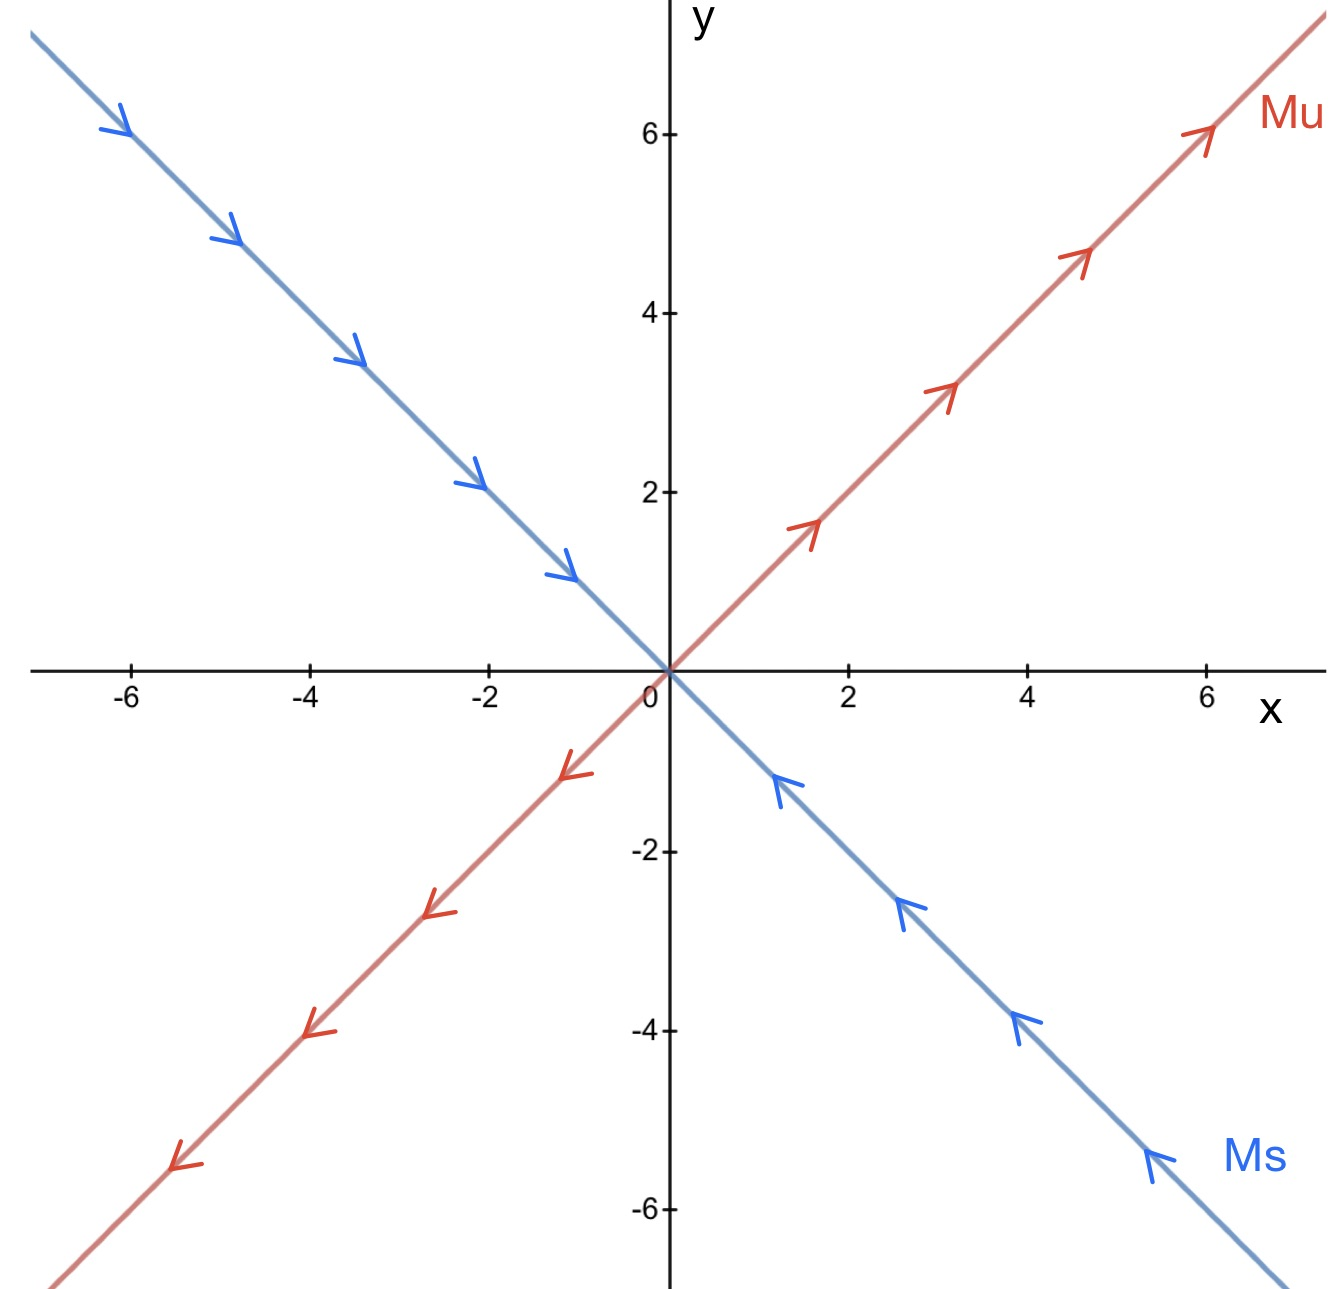
\includegraphics[width=0.4\linewidth]{IMG_0735.jpeg}
    \caption{Cross-section for $z = z_0$}
    \label{fig:stable}
\end{figure}
We can confirm this behavior numerically. We let $(x_0, y_0, z_0) = (-0.01, 0.01, 100)$ with $d = 1$, $f_1 = 1$, $f_3 = 1$, and run the simulation from $t= 0$ to $t = 300$ we get figure \ref{fig:new4}

\begin{figure}[h!]
\centering
\begin{subfigure}{.5\textwidth}
  \centering
  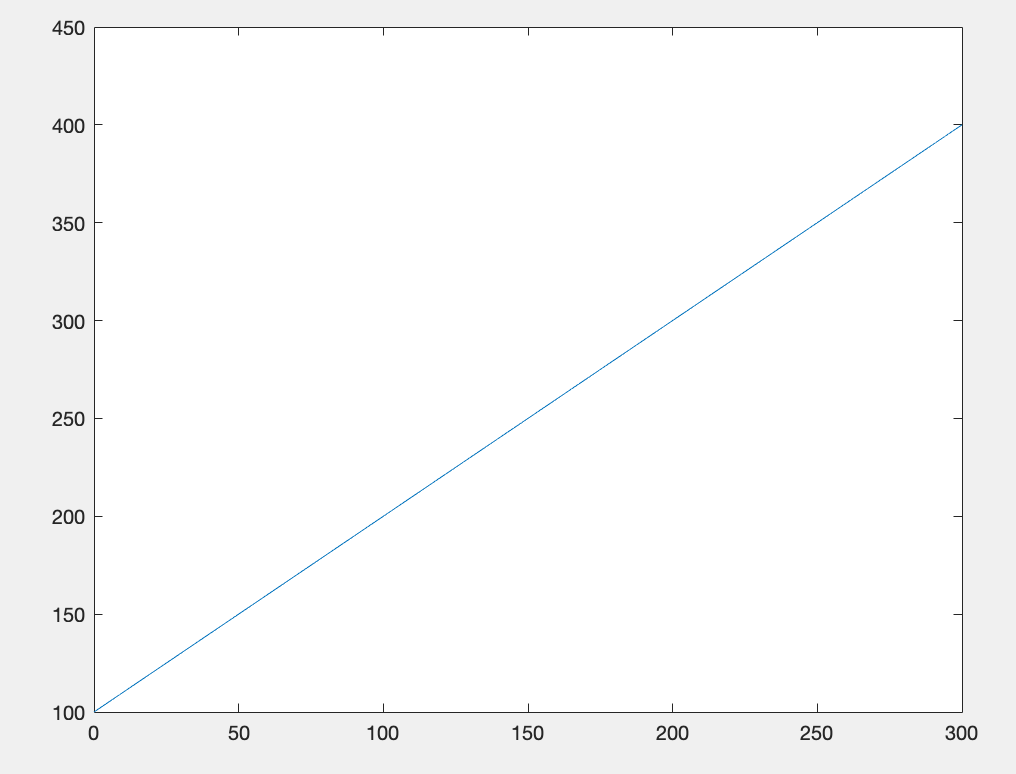
\includegraphics[width=0.9\linewidth]{new4e.png}
  \caption{Energy of the trajectory over time}
  \label{}
\end{subfigure}%
\begin{subfigure}{.5\textwidth}
  \centering
  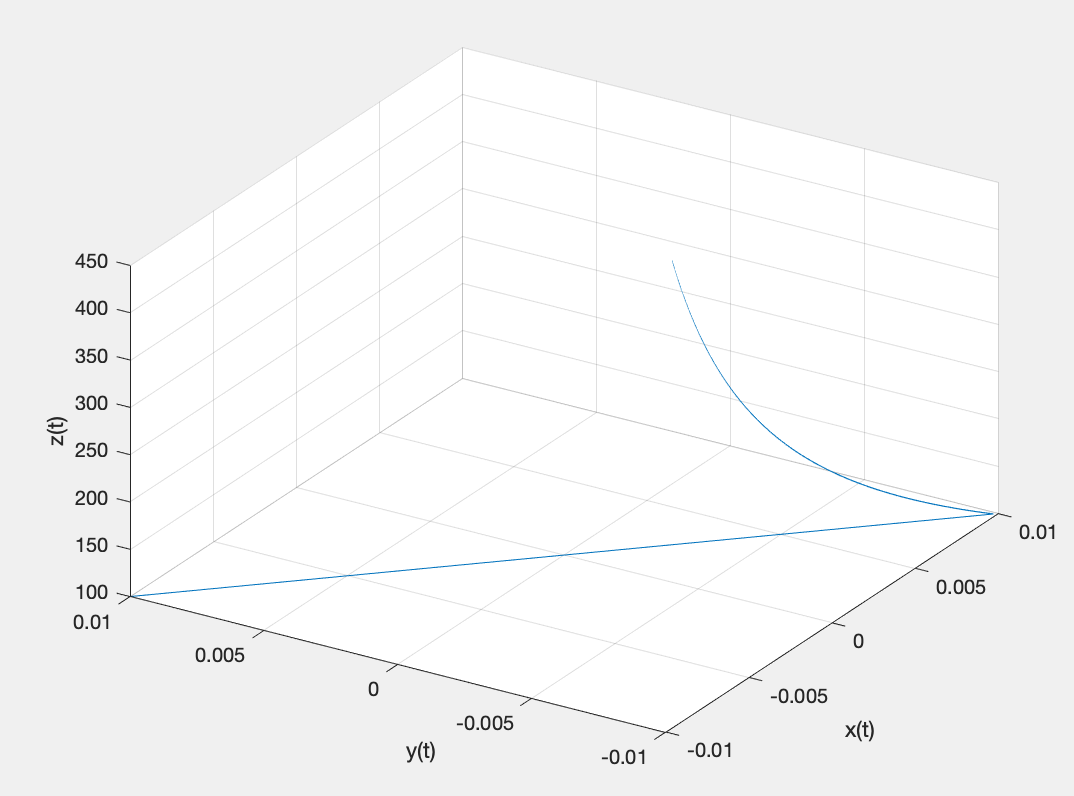
\includegraphics[width=0.92\linewidth]{new4p.png}
  \caption{Plot of trajectory}
  \label{}
\end{subfigure}
\caption{}
\label{fig:new4}
\end{figure}
We notice how the trajectory stays on the stable manifold, and the energy grows at an almost constant rate. 

Since the equilibria of $\psi = 0$ is unstable, in order for divergence to occur the initial conditions must be exactly on the stable manifold of the cross-section. This tells us that our claim could still remain true for initial conditions and forcing without this symmetry. Below in figure \ref{fig:test} we plot the energy of the system over time on the left and the trajectory on the right of \eqref{eq:counterex} with $z(0) = 1000, x(0) = 1, y(0) = -0.99999, f_1 = 1, f_3 = 1, a = 1$ from $t = 0$ to $t = 100$. 




\begin{figure}[h!]
\centering
\begin{subfigure}{.5\textwidth}
  \centering
  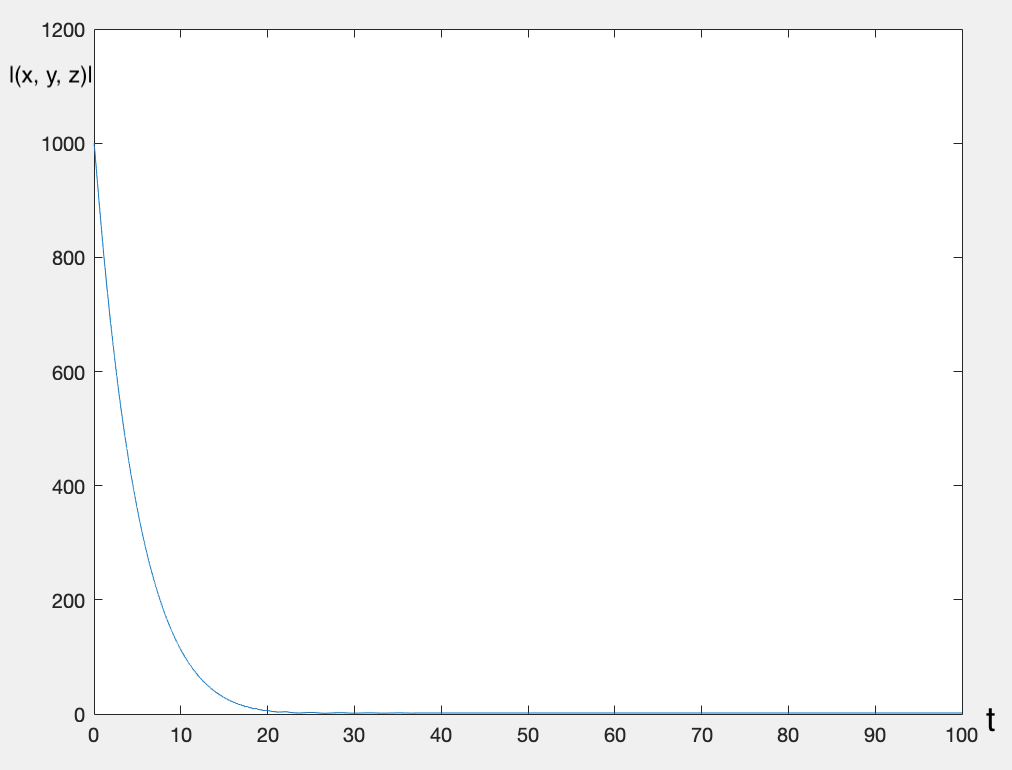
\includegraphics[width=0.9\linewidth]{energy.png}
  \caption{Energy of the trajectory over time}
  \label{fig:sub1}
\end{subfigure}%
\begin{subfigure}{.5\textwidth}
  \centering
  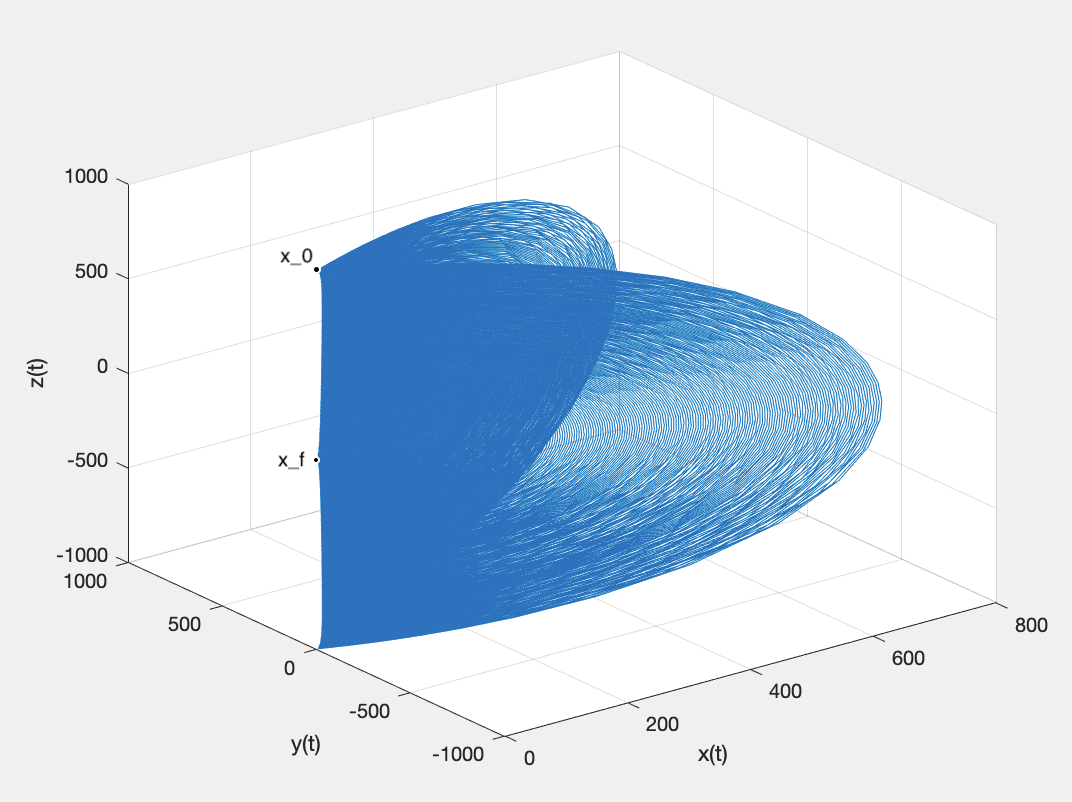
\includegraphics[width=0.9\linewidth]{stable}
  \caption{Plot of trajectory}
  \label{fig:sub2}
\end{subfigure}
\caption{}
\label{fig:test}
\end{figure}

The trajectory oscillates while exponentially losing energy and then falling to a constant low energy in finite time, thus remaining bounded. 


\subsection{Boundedness for Hyperbolic Systems}
We will sketch a proof that the ODE
\begin{equation}\label{eq:last}
    \frac{d}{dt} \begin{pmatrix} x \\ y \\ z 
    \end{pmatrix} = \begin{pmatrix}
        yz - x + 1\\
        xz - y\\
        -2xy + 1\\
    \end{pmatrix} 
\end{equation} remains bounded. There still remains an unfinished approximation argument to complete this proof.\\

We begin by showing that a certain condition is sufficient to show that all solutions to the ODE remain bounded.

\begin{lemma}\label{lem:1}
    Suppose that there exists some $E \in \R$ such that for every $|\mathbf{x}_0| > E$, there is some $T(\mathbf{x}_0) \leq 1$ such that $|\mathbf{x}(T(x_0))| < E$. Then our solution $\mathbf{x}(t)$ remains bounded
\end{lemma}
\textbf{Proof: }Suppose that for every $|\mathbf{x}_0| > E$, there is some $T(\mathbf{x}_0) \leq 1$ such that $|\mathbf{x}(T(x_0))| < E$. Since $$\dv{}{t}|\mathbf{x}(t)|^2 = -x(t)^2 - y(t)^2 + x(t) + z(t)$$it follows that 
\begin{align*}
    \dv{}{t}|\mathbf{x}(t)| &= \frac{-x(t)^2 - y(t)^2 + x(t) + z(t)}{2|\mathbf{x}(t)|}\\
    &\leq \frac{x(t) + z(t)}{2|\mathbf{x}(t)|}\\
    & \leq 1
\end{align*}
Then on our interval $(0, T(x_0))$, the energy can achieve a maximum of $|\mathbf{x}_0| + 1$. And on the interval $(T(x_0), 2T(x_0))$, the solution can only reach a maximum of $E + 1 \leq |\mathbf{x}_0| + 1$. Continuing this process, we have the upper bound $$\underset{t \rightarrow \infty}{\limsup} |\mathbf{x}(t)| < E + 1$$or that our solution remains bounded. 

The following sketch of a proof aims to show that the conditions of lemma \ref{lem:1} are met, but lacks the approximation argument to complete the proof. Soon, I hope to have the approximation argument complete and the whole proof done. 

We will prove this condition is met by partitioning $\R^3$ into the three sets $M_1 \cup M_2 \cup M = \R^3$, showing that solutions in $M_1$ will enter $M_2$ in short time, that solutions in $M_2$ will enter $M$ in short time, and solutions in $M$ with energy greater than $E$ will satisfy the condition of lemma \ref{lem:1}. We define
\begin{align*}
    M &= \{ \mathbf{x} \in \R^3 \, : \, |x|^2 + |y|^2 \geq \delta |z|^2 \}\\
    M_1 &= \{ \mathbf{x} \in \R^3 \, : \, |x|^2 + |y|^2 \leq |z|^{-2} \}\\
    M_2 &= (M \cup M_1)^c
\end{align*}
First, we will prove that for some $E>0$, all points such that $|\mathbf{x_0}| > E$ and are in $M$ must lose $c\sqrt{ E}$ energy in a small time $t < T'$ for some $c\in \R$. Then there must be some $1/3> T_3 \geq T'$ such that in a time $t < T_3$ we have $|\mathbf{x}(t)| < E$. Then we will show that for all $\mathbf{x}_0 \in M_1$, the solution will enter $M_2$ in some $t < T_1$, for all $\mathbf{x}_0 \in M_2$, the solution will enter $M$ in some time $t < T_2$. Together, this will give us that for all $|\mathbf{x}_0| > E$, in some $T^* < T_1 + T_2 + T_3 < 1$, the condition that $|\mathbf{x}(T^*)| < E$ is met and we conclude the proof.

Without loss of generality, we let $$|x_0| \geq |y_0|$$and note that in $M$:
\begin{align*}
    E &\leq \sqrt{|x_0|^2 + |y_0|^2 + |z_0|^2}\\
    & \leq \sqrt{|x_0|^2 + |x_0|^2 + \frac{2}{\delta}|x_0|^2}\\
    & \leq |x_0|\sqrt{2 + \frac{2}{\delta}}
\end{align*}
 And denoting $c_{\delta} = (2 + \frac{2}{\delta})^{-1}$, we have that $$|x_0| \geq c_{\delta}E$$First, we will prove the following lemma:
 \begin{lemma}
     There exists some $\epsilon > 0$ that is dependent only on $\delta$ such that if $t \leq \frac{\epsilon}{E}$, then $|x(t)| \geq \frac{1}{2}|x_0|$
 \end{lemma}\\

 \textbf{Proof:} We will prove this using a Taylor expansion. For some $s \in (0, t)$, we can write $x(t)$ as follows. 
 \begin{align*}
     x(t)&= x_0 + t(y_0z_0 - x_0 + 1) + \frac{t^2}{2}(-y(s)z(s) + x(s) - 1)\\
     &+ \frac{t^2}{2}(y(s)(-2x(s)y(s)+1) + z(s)(x(s)z(s)-y(s)))\\
     |x(t)| &\geq |x_0| - t(|y_0z_0 - x_0 + 1|) - \frac{t^2}{2}(|y(s)z(s) + x(s) - 1|)\\
     &- \frac{t^2}{2}(|y(s)(-2x(s)y(s)+1) + z(s)(x(s)z(s)-y(s))|)\\
     & \geq |x_0| - tc_1E^2 - t^2c_2E^3
 \end{align*}
 For some $c_1, \, c_2, \, c_3> 0$ as we know that $s < \frac{\epsilon}{E} << 1$. Then, using $|x_0| \geq c_{\delta}E$, we have that 

 \begin{align*}
    |x(t)| &\geq |x_0| - c_1\epsilon E - c_2 \epsilon^2 E\\
    &\geq |x_0| - c_3\epsilon c_\delta |x_0|\\
    & \geq |x_0|(1 - c_3 \epsilon c_{\delta})
 \end{align*}

Then, there must be a $\epsilon$ dependant only on $\delta$ such that $1 - c_3 \epsilon c_{\delta} < 1/2$, concluding the proof of our lemma. \\

Now for $t \in I$ where $I = (0, \frac{\epsilon}{E})$, we can bound the change in energy
\begin{align*}
    \dv{}{t}|\mathbf{x}|^2 &= -\frac{1}{2}|x(t)|^2 - \frac{1}{2}|y(t)|^2 + \frac{1}{2}|x(t)| + \frac{1}{2}|z(t)|\\
    &\leq -|x(t)|^2 + 2E\\
    & \leq \frac{-|x_0|^2}{8} + E\\
    & \leq -\frac{c_{\delta}^2E^2}{8} + E\\
    &\leq E\left(\frac{-c_{\delta}^2E}{8} + 1\right)
\end{align*}
Letting $k = \frac{c_{\delta}^2E}{8} - 1 > 0$, if $|\mathbf{x_0}|^2 \geq E^2$, then  
\begin{align*}
    \left|\mathbf{x}\left(\frac{\epsilon}{E}\right)\right|^2 - |\mathbf{x}_0|^2 &\leq \int_I -Ek \, dt \\
    &\leq -Ek (\frac{\epsilon}{E}) \\
    &\leq -\frac{c_{\delta}^2E\epsilon}{8} + \epsilon 
\end{align*}
Then we conclude that on our interval of $I$, our energy must decrease by at least $c_{\delta}\sqrt{\frac{E\epsilon}{8}}$. Then, if we let $T^* = \frac{\epsilon}{E} << 1$, we have shown that for some $t < T^*$, $$|\mathbf{x}(t)| < |\mathbf{x}_0| - c_{\delta}\sqrt{\frac{E\epsilon}{8}}$$ Then for some $t < nT^* < 1/3$, we can use the fact that $\dv{}{t}\mathbf{x}(t) \leq 1$ to show that $|\mathbf{x}(t)| < E$ when $n$ is defined as $$n = \frac{8(|\mathbf{x}_0| - E)}{c_{\delta}\sqrt{E\epsilon}}$$Then we let $T_3 = nT^*$ and conclude that for some $t < T_3 < 1/3$, our $|\mathbf{x}(t)| < E$ as desired. 

Now we show that solutions with initial conditions $\mathbf{x}_0 \in M_1$ enter $M_2$ in a short time. The method of projecting the solution onto the unit sphere and then studying the dynamics on this sphere, which would have the linearization of a saddle near the point $(0, 0, 1)$, on the tangent plane with the approximation $z(t) = z_0$ would not work as there would exist a fixed point and a stable manifold in the linearization that threatens boundedness. We will briefly show this. 

Supposing that for small $x_0, y_0$ we approximate $z(t) = z_0$. We then have the ODE in the $xy$-plane:
\begin{equation*}
    \begin{cases}
        \displaystyle
        \dot{x} = yz_0 - x + 1\\

        \displaystyle
        \dot{y} = xz_0 - y
    \end{cases}
\end{equation*}
This of course has a fixed point at $$(x^*, y^*, z^*) = \left( \frac{-1}{z_0^2 - 1}, \frac{-1}{z_0-\frac{1}{z_0}}, z_0 \right)$$which does not support our claim that our solution must leave $M$. 

Instead, for $\mathbf{x}_0$ very close to the $z$-axis we must approximate $\dot{z}(t) = 1 $ which gives us the solution $z(t) = z_0 + t$. This makes our approximation the non-autonomous ODE
\begin{equation}\label{eq:nonauto}
\begin{cases}
    \displaystyle
    \dot{x} = yz_0 + tx - x + 1\\

    \displaystyle
    \dot{y} = xz_0 + ty - y
\end{cases}
\end{equation}
Now we claim that initial conditions $\mathbf{x}_0 \in M_1$ must leave $M_1$ in a small time $T_1 < 1/3$. We will do so by introducing a new variable, finding an explicit solution to \eqref{eq:nonauto} using an integrating factor, and then approximating the resulting integral with a Taylor expansion. 

As we did in section 3.1, let $$\psi(t) = x(t) + y(t)$$then, substituting this into \eqref{eq:nonauto}, we have the ODE 
\begin{equation*}\label{eq:nonautosum}
    \dot{\psi}(t) = (z_0 - 1 +t)\psi(t) + 1 
\end{equation*}
Note that unlike the example in section 3.1 $\psi_0 = 0$ is not a fixed point. Now we rewrite \eqref{eq:nonautosum} as $$\dot{\psi}(t) + (-z_0 + 1 -t)\psi(t) = 1 $$and get our integrating factor of $\exp(\int- (z_0 - 1 +t) dt ) = \exp(t(-z_0 + 1) - t^2/2)$. We multiply both sides by the integrating factor and integrate to get
\begin{align*}
    \int e^{t(-z_0 + 1) - t^2/2}\psi'(t)dt  +\int e^{t(-z_0 + 1) - t^2/2}\psi(t)(-z_0 + 1 - t)dt &= \int e^{t(-z_0 + 1) - t^2/2}dt
\end{align*}
Then we can integrate the first term on the left hand side by parts to get 
\begin{align*}
    \int e^{t(-z_0 + 1) - t^2/2}\psi'(t)dt = e^{t(-z_0 + 1) - t^2/2}\psi(t) - \psi(0) - \int e^{t(-z_0 + 1) - t^2/2}\psi(t)(-z_0 + 1 - t)dt
\end{align*}
which, when we substitute back into the previous expression yields 
\begin{align*}
    e^{t(-z_0 + 1) - t^2/2}\psi(t)  &= \int e^{t(-z_0 + 1) - t^2/2}dt + \psi(0) 
\end{align*}
which with some manipulation yields the expression
\begin{align*}
    \psi(t) &=e^{t(z_0 - 1) + t^2/2} \left(\int_0^{t} e^{s(-z_0 + 1) - s^2/2}ds + \psi(0)\right)\\
    &= e^{t(z_0 - 1) + t^2/2}\left( \int_0^t e^{s(-z_0 + 1)} e^{- s^2/2}ds + \psi(0)\right)
\end{align*}
Now since we are working on a timescale which is very small, we replace the term $e^{- s^2/2}$ with its Taylor expansion around $s = 0$, giving us the approximation $e^{- s^2/2} = 1 - \frac{s^2}{2} + O(s^4)$. We ignore the terms greater than order four, and substituting the Taylor expansion into our equation we have $$\psi(t) = e^{t(z_0 - 1) + t^2/2} \int_0^t e^{s(-z_0 + 1)}\left(1 - \frac{s^2}{2}\right)ds + \psi(0)e^{t(z_0 - 1) + t^2/2}$$which we can integrate by parts as follows
\begin{align*}
    \int_0^t e^{s(-z_0 + 1)}\left(1 - \frac{s^2}{2}\right)ds &= \left[ e^{s(-z_0 + 1)}\left( \frac{1}{-z_0 + 1}\right) \left( 1 - \frac{s^2}{2} \right)\right]\bigg\rvert_{s = 0}^t   + \int_0^t se^{s(-z_0 + 1)}ds
\end{align*}
Then we evaluate 
\begin{align*}
    \int_0^t se^{s(-z_0 + 1)}ds &= \left[ \frac{s}{1- z_0} e^{s(-z_0 + 1)} \right]\bigg\rvert_{s = 0}^t - \int_0^t \frac{1}{1 - z_0}e^{s(1 - z_0)}ds\\
    &= \frac{t}{1- z_0} e^{t(-z_0 + 1)} - \left[ \frac{1}{(1-z_0)^2}e^{s(1 - z_0)} \right]\bigg\rvert_{s = 0}^t \\
    &= \frac{t}{1- z_0} e^{t(-z_0 + 1)} -  \frac{1}{(1-z_0)^2}\left(e^{t(1 - z_0)} - 1\right) 
\end{align*}
Which, when we plug back into the earlier equation, we get
\begin{align*}
    \int_0^t e^{s(-z_0 + 1)}\left(1 - \frac{s^2}{2}\right)ds &= \frac{e^{t(1-z_0)}\left( 1 - \frac{t^2}{2} \right) - 1}{1 - z_0} + \frac{t}{1- z_0} e^{t(-z_0 + 1)} -  \frac{\left(e^{t(1 - z_0)} - 1\right)}{(1-z_0)^2}
\end{align*}
Finally, we have the solution
\begin{align*}
    \psi(t) &=\frac{e^{t(z_0 - 1) + t^2/2}}{1-z_0}\left(e^{t(1-z_0)}\left( 1 - \frac{t^2}{2} \right) - 1 + t e^{t(-z_0 + 1)} -  \frac{\left(e^{t(1 - z_0)} - 1\right)}{1-z_0} + \psi(0)(1-z_0) \right)
\end{align*}
Now, we can perform more Taylor expansions to yield $e^{t(z_0 - 1) + t^2/2} = e^{t(z_0 - 1)}(1 + t^2/2)$, which when substituted into the above equation yields 
\begin{align*}
    \psi(t) &= \frac{e^{t(z_0 - 1)}(1 + t^2/2)}{1-z_0}\left(e^{t(1-z_0)}\left( 1 - \frac{t^2}{2} \right) - 1 + t e^{t(-z_0 + 1)} -  \frac{\left(e^{t(1 - z_0)} - 1\right)}{1-z_0} + \psi(0)(1-z_0) \right)\\
    &= (1-z_0)^{-1}\left(1 - t^4/4 - e^{t(z_0 - 1)}(1 + t^2/2) + t(1 + t^2/2) - \frac{(1 + t^2/2)(1 - e^{t(z_0 - 1)})}{1-z_0} \right)\\ &\qquad \qquad  + e^{t(z_0 - 1)}(1 + t^2/2)\psi(0)
\end{align*}
For small time, we notice that the first term on the RHS is of a lower order than the second as it is multiplied by $(1-z_0)^{-1}$. But, we also note that it is this term that ensures that there is no fixed point for $\psi(0) = 0$ that may lead to divergence as seen in section 3.1. So we know that we will move off of any potential stable manifold, and can assume that $\psi(0) \neq 0$ in our apporximations. 

Also, we note that since the forcing is in the positive $z$-direction, our solution can only diverge along the $z$-axis to $z = +\infty$, so we are assuming that $z_0 > 0$. With both of these properties in mind, we can assume $\psi(0) \neq 0$ and make the following approximations for a very small $t > 0$. 
\begin{align*}
    |\psi(t)| &\geq \frac{e^{t(z_0 - 1)}|\psi(0)|}{2} 
\end{align*}
In order to leave $M_1$ at some $t$, we must have $$|x(t)| + |y(t)| \geq |\psi(t)| \geq |z|^{-1} \geq E^{-1}$$which occurs at some $t < T_1$ when $$E^{-1} = \frac{e^{T_1(z_0 - 1)}|\psi(0)|}{2}$$we evaluate that our solution must leave $M_1$ at some $t < T_1$ for $$T_1 = \frac{\ln\left(\frac{2}{E|\psi(0)|} \right)}{z_0 - 1} << 1/3$$

Now that we have show that all solutions leave $M_1$ in short time, we will show that all solutions with $|\mathbf{x_0}| > E$ such that $\mathbf{x_0} \in M_2$ will leave $M_2$ in short time. Also, suppose that either $|x_0| \geq \frac{2}{E}$ or $|y_0| \geq \frac{2}{E}$ or both do.

As we did in our proof that the unforced case must converge to the origin, we let $u(t) = \pi_{\ker A^{\perp}} x(t)$, so that $u(t)$ is the distance from the solution to the $z$-axis, and again we have $z_0 > E$. Now with our assumptions of $|x_0|$ and $|y_0|$, we can study the dynamics of the projection of this system onto the unit sphere. In doing so we must also scale time. We introduce $\tau = |\mathbf{x}_0|t \sim z_0t$ and $\widetilde{\mathbf{x}} = \frac{\mathbf{x}}{\abs{\mathbf{x}}}$. Then our ODE becomes 
\begin{equation}\label{eq:proj}
    \dv{}{t}\widetilde{\mathbf{x}} = B(\widetilde{\mathbf{x}}, \widetilde{\mathbf{x}}) - \frac{1}{z_0}A\widetilde{\mathbf{x}} + \frac{1}{z_0^2}f
\end{equation}
with $\widetilde{z_0} \sim 1$. We also notice that with scaling $M$ remains unchanged, and so does the result we are trying to prove that we must leave $M$ in short time. 

Since $z_0 >> 1$ and $\widetilde{x_0}, \widetilde{y_0}<< 1$, we approximate the dynamics as 
\begin{equation}\label{eq:approx}
\begin{cases}
\displaystyle
\dot{\widetilde{x}} = \widetilde{y}\widetilde{z}\\

\displaystyle
\dot{\widetilde{y}} = \widetilde{x}\widetilde{z}\\

\displaystyle
\dot{\widetilde{z}} = -2\widetilde{x}\widetilde{y}
\end{cases}
\end{equation}
in which we ignore both forcing and damping due to the scaling. Then we make the next approximation that $\widetilde{x}\widetilde{y} \sim 0$ inside $M$, leaving us with $\dot{\widetilde{z}} \sim 0$ and $\widetilde{z}(t) = \widetilde{z_0} \sim 1$. Then our new system is
\begin{equation}\label{eq:onplane}
\begin{cases}
\displaystyle
\dot{\widetilde{x}} &= \widetilde{y}\\

\displaystyle
\dot{\widetilde{y}} &= \widetilde{x}
\end{cases}
\end{equation}
which is just a saddle on the plane $z = 1$ tangent to the unit sphere. The dynamics are shown in figure \ref{fig:proj} below. 

\begin{figure}[h!]
    \centering
    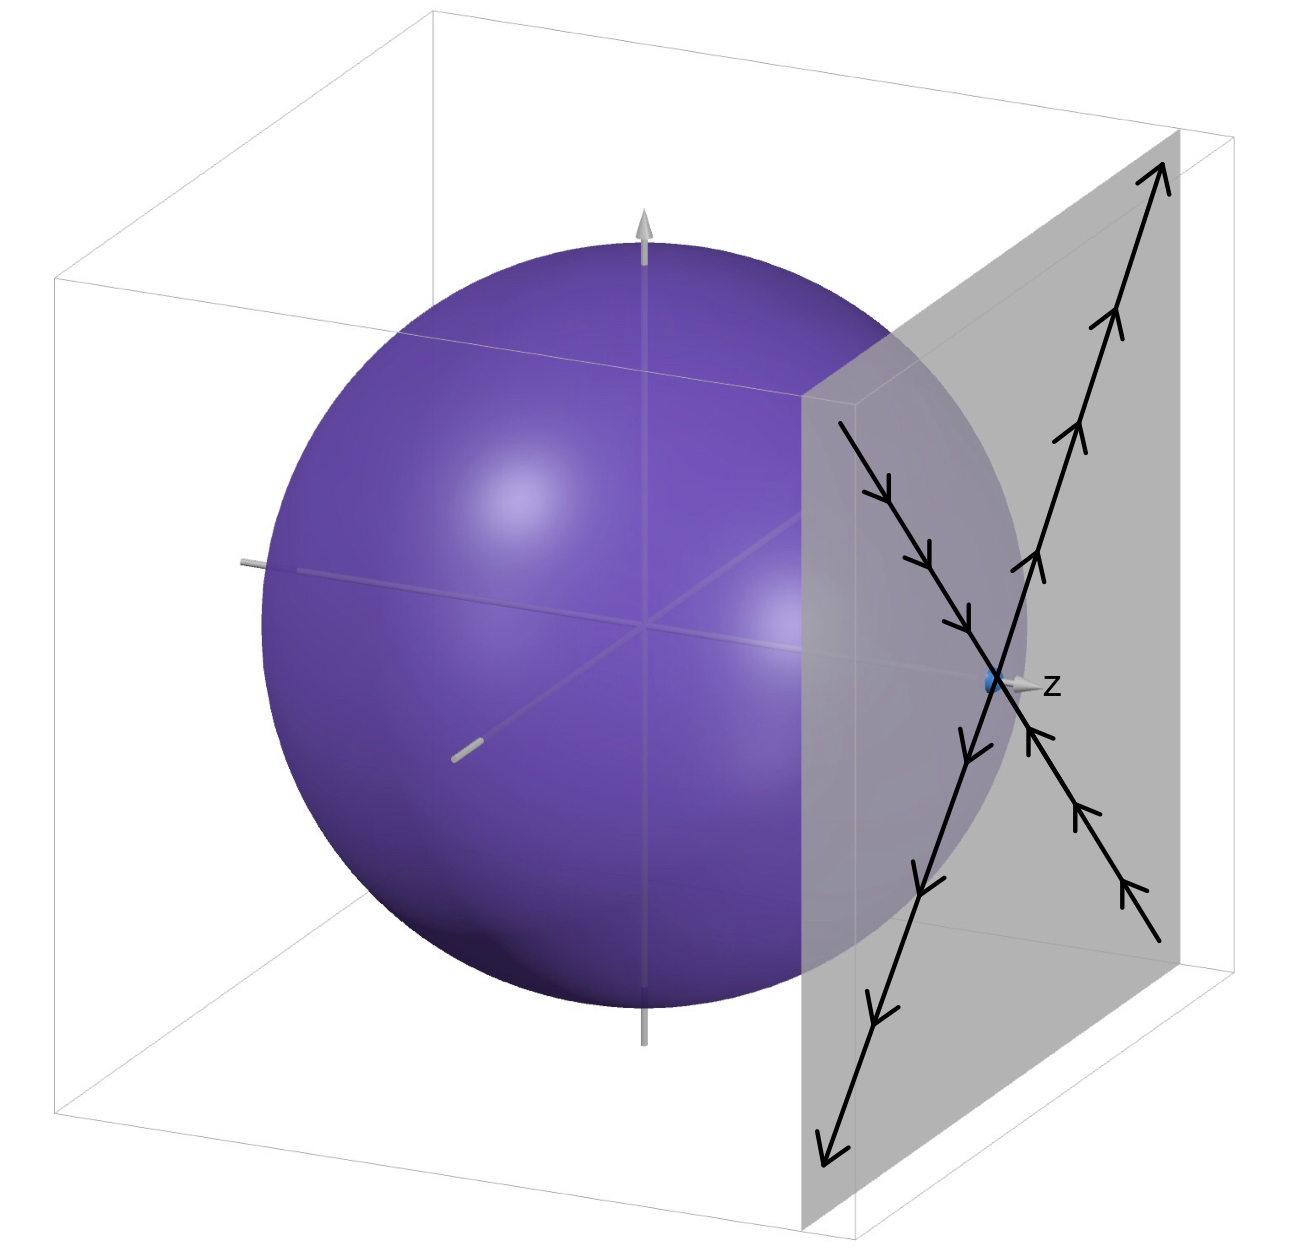
\includegraphics[width=0.4\linewidth]{proj.jpeg}
    \caption{}
    \label{fig:proj}
\end{figure}
Let us suppose that $x_0, y_0 > 0$ and $|\widetilde{u_0}| = \frac{u_0}{|\mathbf{x_0}|}$. Thus, we can make the assumption that $\widetilde{x_0}, \widetilde{y_0} > 0$ and $$\widetilde{u_0} = \frac{1}{z_0}$$where $\widetilde{u} = \pi_{\ker A^{\perp}}\widetilde{\mathbf{x}}$ and $|u| = (x^2 + y^2)^{1/2}$. Solving \eqref{eq:onplane} yields the solution
\begin{equation}\label{eq:solution}
\begin{cases}
\displaystyle
\widetilde{x(\tau)} = \frac{\widetilde{x_0}}{2}(e^{\tau} + e^{-\tau}) + \frac{\widetilde{y_0}}{2}(e^{\tau} - e^{-\tau})\\

\displaystyle
\widetilde{y(\tau)} = \frac{\widetilde{x_0}}{2}(e^{\tau} - e^{-\tau}) + \frac{\widetilde{y_0}}{2}(e^{\tau} + e^{-\tau})
\end{cases}
\end{equation}on the plane. Then it follows that 
\begin{align*}
    |\widetilde{u}(\tau)|^2 &= |\widetilde{x}(\tau)|^2 + |\widetilde{y}(\tau)|^2\\
    &= \frac{\widetilde{x}_0^2 + \widetilde{y}_0^2}{2}(e^{2\tau} + e^{-2\tau})\\
    &= \frac{\widetilde{u}_0^2}{2}(e^{2\tau} + e^{-2\tau})\\
    & < \frac{\widetilde{u}_0^2}{2}(e^{2\tau})
\end{align*}Now, we want to find some $\tau^*$ such that $\widetilde{\mathbf{x}}$ leaves $M_2$, which will happen when $|\widetilde{u}(\tau^*)|^2 > \delta |z_0|^2$, or at 
\begin{align*}
    \frac{(\widetilde{u}_0e^{\tau^*})^2}{2} &= \delta |z_0|^{2}\\
    \tau^* &= \ln\left(\frac{\sqrt{2}\delta |z_0|}{|\widetilde{u_0}|}\right)
\end{align*}
Noting that $|\widetilde{u_0}| > |z_0|^{-1}$, we are left with
\begin{align*}
    \tau^* &< \ln\left(\sqrt{2}\delta |z_0|^2\right)\\
    &< 2\ln (2^{1/4}\sqrt{\delta}|z_0|)
\end{align*}
Finally rescaling time, we have that $\mathbf{x}$ must leave $M$ at some time $t = t^*$ such that $$t^* < \frac{2\ln (2^{1/4}\sqrt{\delta}|z_0|)}{|z_0|} << 1$$Then we can define $T_2 = t^* < 1/3$, concluding that if $T^* < T_1 + T_2 + T_3 < 1$, and $|\mathbf{x_0}| > E$, then at some time $t < T^*$ our solution $|\mathbf{x}(t)| < E$ and thus remains bounded by lemma \ref{lem:1}. 

\subsection{Boundedness for Elliptic Systems}

In this section, we will consider the ODE\begin{equation}\label{eq:elliptic2}
    \frac{d}{dt} \begin{pmatrix} x \\ y \\ z 
    \end{pmatrix} = \begin{pmatrix}
        ayz\\
        bxz\\
        -(a+b)xy
    \end{pmatrix} - \begin{pmatrix}
        d_1 & 0 & 0 \\
        0 & 0 & 0 \\ 
        0 & 0 & d_3 
    \end{pmatrix} \begin{pmatrix} x \\ y \\ z 
    \end{pmatrix} 
    + 
    \begin{pmatrix} f_1 \\ f_2 \\ f_3
    \end{pmatrix}
\end{equation}with $a, b, d_1, d_3 > 0$. As discussed earlier in this section, for $y_0>>1$ we expect the dynamics in the cross sections of the $xz$-plane to exhibit center like behavior around the $y$-axis. Figure \ref{fig:parab} below depicts the expected behavior contributed from the bilinear term $B$.
\begin{figure}[h!]
    \centering
    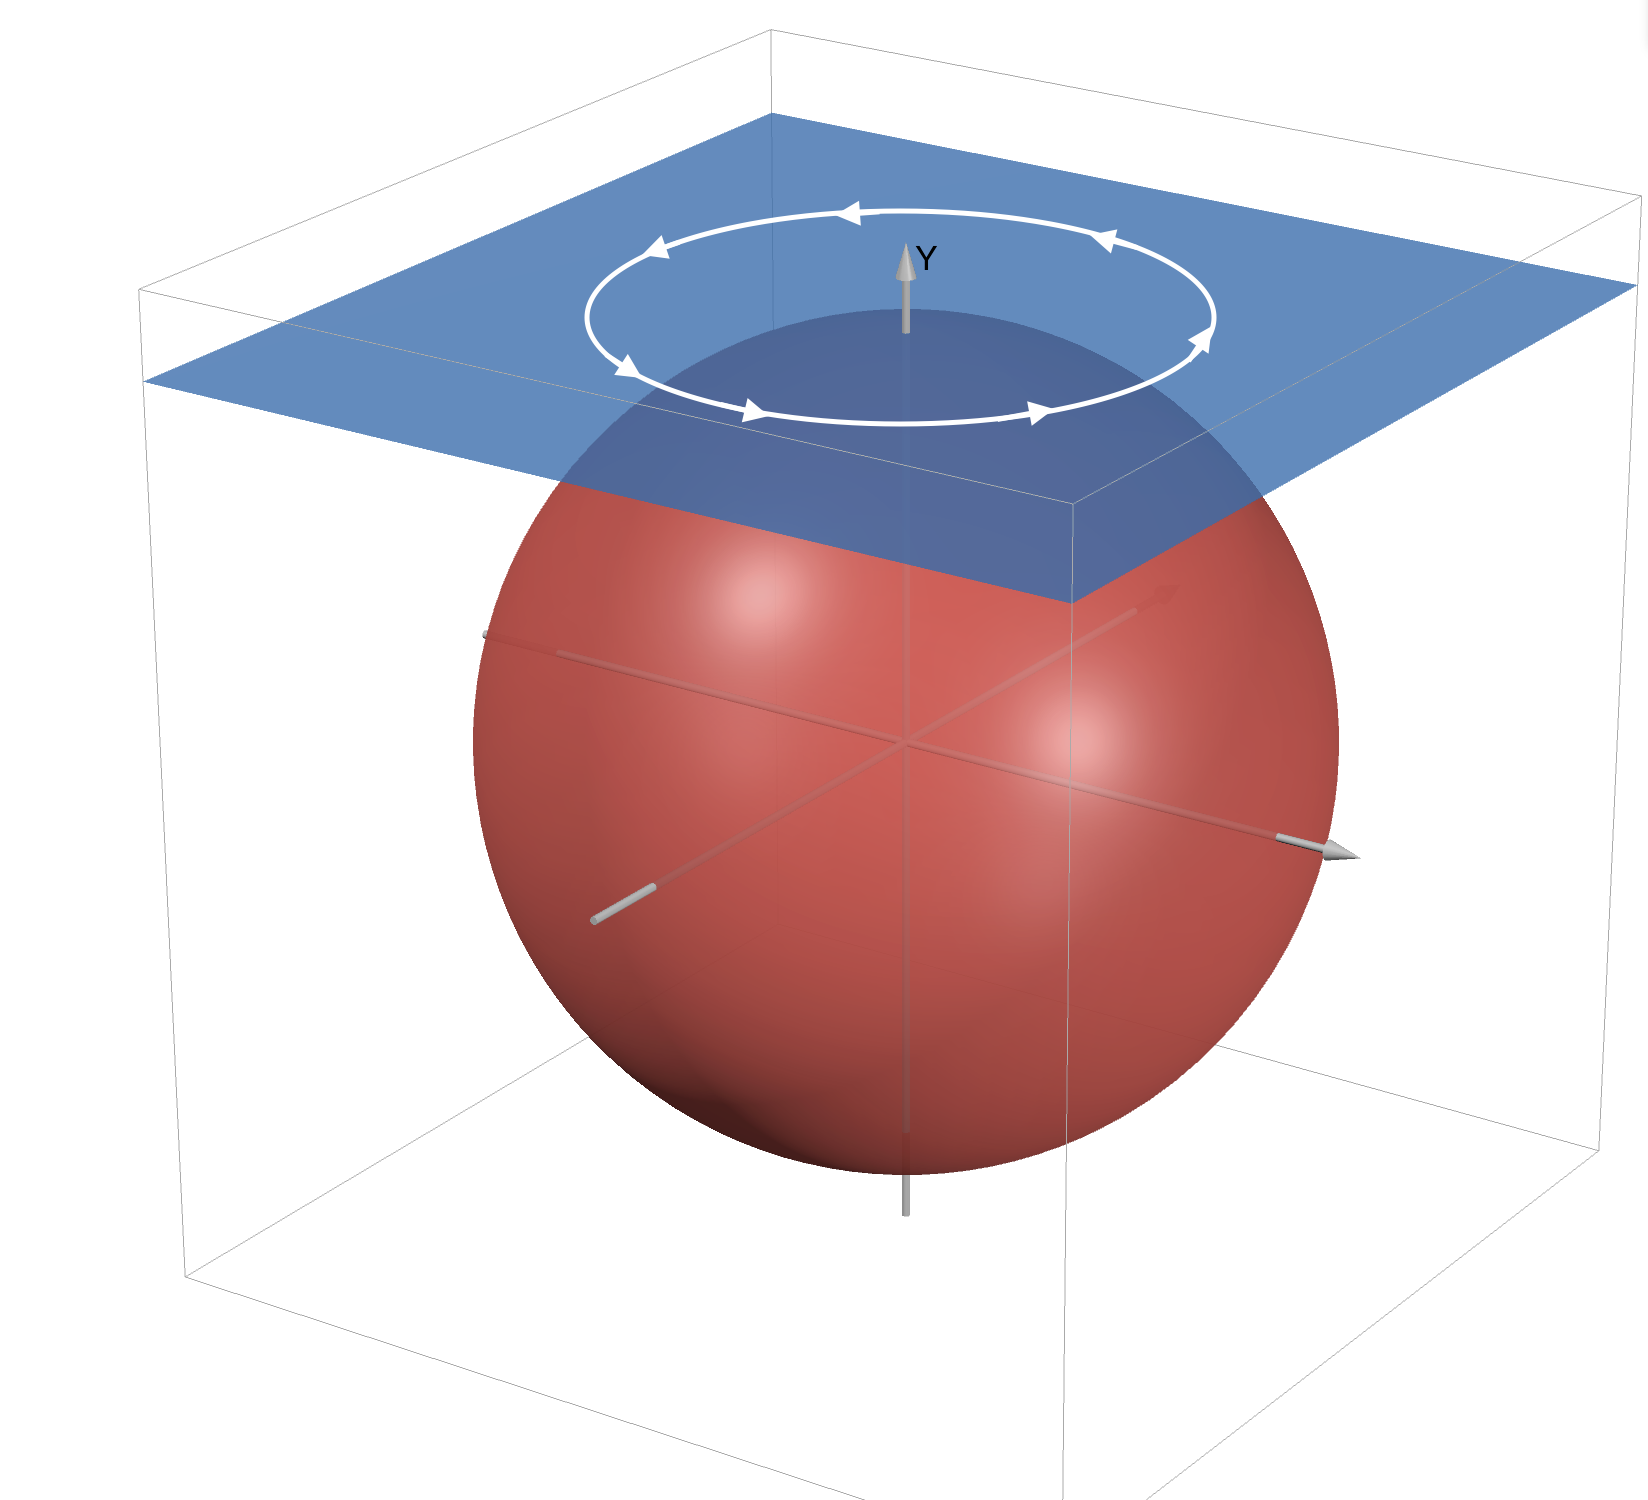
\includegraphics[width=0.4\linewidth]{parab.png}
    \caption{The linearization of an elliptic fixed point on the $y$-axis}
    \label{fig:parab}
\end{figure}


Note that the region $M$ for which the energy of the system is increasing will be similar in shape to that used in the previous subsection on hyperbolic fixed points, only now it is oriented on the $y$-axis and is dependant on our matrix $A$ and the forcing. As the $y$-axis hosts stable equilibria, we assume that there will be trajectories in which the conservative term cause the trajectory to spiral inside $M$ while gaining energy from the forcing term, eventually diverging to infinity. We will show an interesting relationship between the presence of fixed points of \eqref{eq:elliptic2} and boundedness. 

We can find the fixed points of \eqref{eq:elliptic2} by first finding the conditions for which $\dot{y} = 0$, which happens when $$x = \frac{-f_2}{bz}$$Then, in order for $\dot{x} = 0$, our parameters must satisfy $ayz = d_1x - f_1$. When our result from $\dot{y} = 0$ is substituted in, we get the relationship $$y = \left(\frac{-d_1f_2 - f_1b}{ab} \right)\frac{1}{z^2}$$Finally, substituting the prior results into $-(a + b)xy + f_3 = d_3z$, we get an expression for the $z$-values of fixed points
\begin{equation}\label{eq:fixedz}
    \frac{-f_2(a + b)(d_1f_2 + f_1b)}{ab^2} + f_3z^3 - d_3z^4  = 0
\end{equation}
To simplify the above equation, we can let $c_1 = d_3$, $c_2 = f_3$, and $c_3 = -f_2(a + b)(d_1f_2 + f_1b)/(ab^2)$ so that $$0 = -c_1z^4 + c_2z^3 + c_3$$Note that $c_1>0$, $c_2 \neq 0$ and $c_3$ has no restrictions. Also, note that for every solution $z$, there is exactly one pair of $(x,y)$ such that $(x,y,z)$ is a fixed point, as indicated in our process of finding \eqref{eq:fixedz}.

Graphing $f(z) = -c_1z^4 + c_2z^3 + c_3$ we notice that any set of parameters $(c_1, c_2, c_3)$ yields either zero, one, or two roots. An example of when this equation has zero real roots is when $c_1 = 5$, $c_2 = -4$, $c_3 = -2$. For ease of calculation, let $a = 1$ and $b = 1$ so that $c_3 = -2f_2(d_1f_2 + f_1)$. To satisfy $c_3 = -1$, we let $f_2 = 1$, $d_1 = 2$ and $f_1 = -1$. Then to satisfy the requirements for $c_2$ and $c_1$ we let $d_3 = 5$ and $f_3 = -4$. Now, as we are trying to find unbounded behavior for the system, we choose initial conditions with a large $y_0$ and very small $x_0, z_0$. We will choose $x_0 = z_0 = 0.01$ and $y_0 = 100$. The results are as follows. 
\begin{figure}[h!]
\centering
\begin{subfigure}{.5\textwidth}
  \centering
  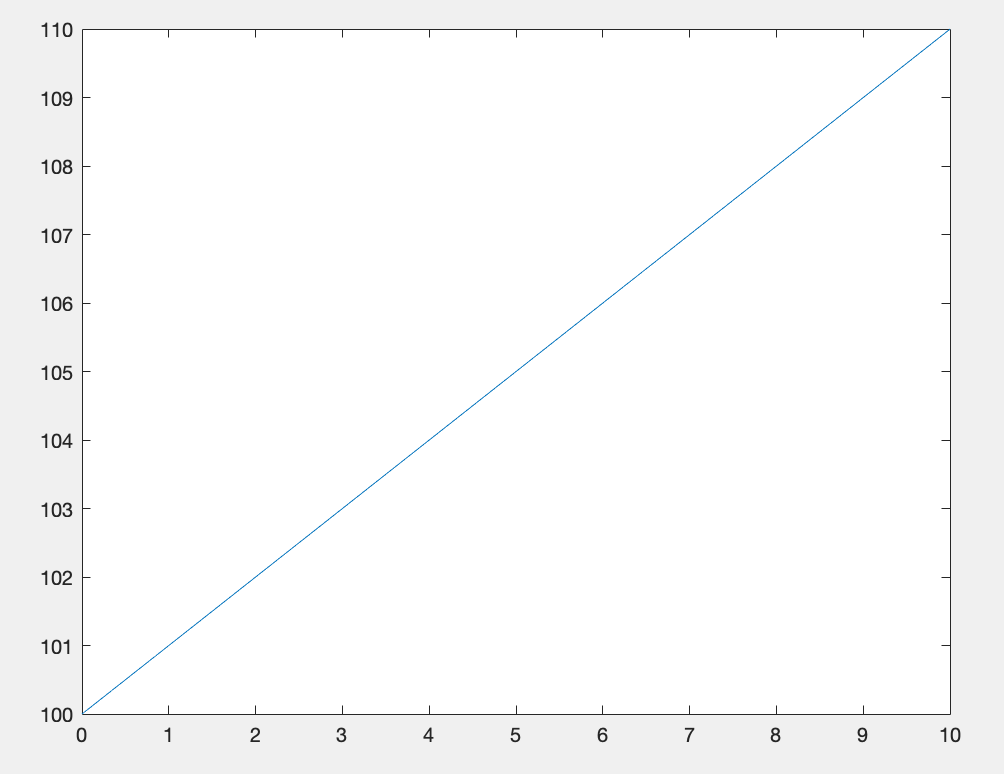
\includegraphics[width=0.9\linewidth]{energy1.png}
  \caption{Energy of the trajectory over time}
  \label{fig:sub1}
\end{subfigure}%
\begin{subfigure}{.5\textwidth}
  \centering
  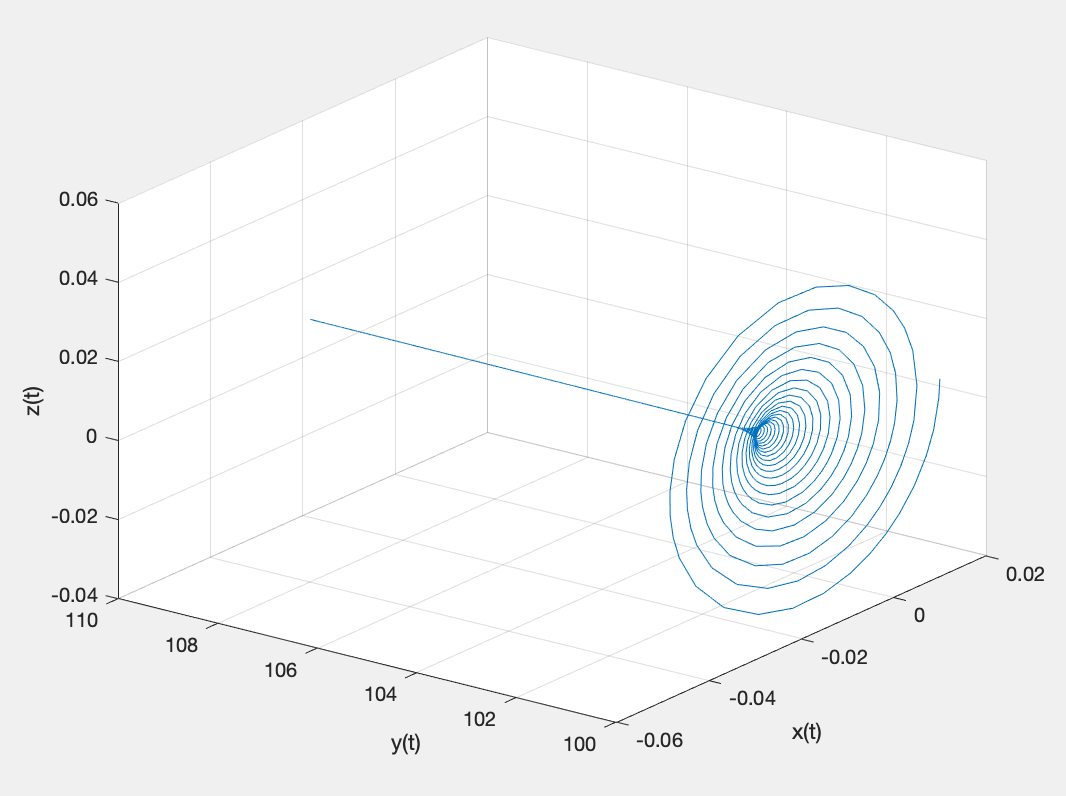
\includegraphics[width=0.924\linewidth]{plot1.png}
  \caption{Plot of trajectory}
  \label{fig:sub2}
\end{subfigure}
\caption{Plots for zero fixed points}
\label{fig:test}
\end{figure}


The trajectory begins at the outer edge of the spiral in plot b and then enters the kernel of $A$ where it diverges to infinity. We choose $y_0 > 0$ as the forcing is in the positive $y$-direction, so must diverge in the positive direction of the $y$-axis. Plots for longer time confirm that this behavior continues and I am only limited by the computation that my laptop permits. Also, as the energy is only being increased by the forcing, it will resemble a linear graph as seen in figure a. Now, we will show that when one fixed point is present, this behavior ceases. 

Now, we can calculate that \eqref{eq:fixedz} has exactly two real roots very close to each other when $c_1 = 5$, $c_2 = 6.978$, and $c_3 = -2$. Note that we have only changed $c_2$, and that for any $c_2$ more than a $0.01$ less than that which was just inputted, we have zero real roots. Then, we use the same parameters as in the last computation, but we must adjust $f_3$. Now, we choose an initial point close to the fixed points, which are near $z^* \sim 0.808$, $x^* \sim −1.24$, $y^* \sim −1.837$. We must truncate these numbers as the simulations in MATLAB fail when so many decimals are included in the initial conditions. The trajectory and energy of the trajectory is plotted below in figure \ref{fig:une}. 

\begin{figure}[h!]
\centering
\begin{subfigure}{.521\textwidth}
  \centering
  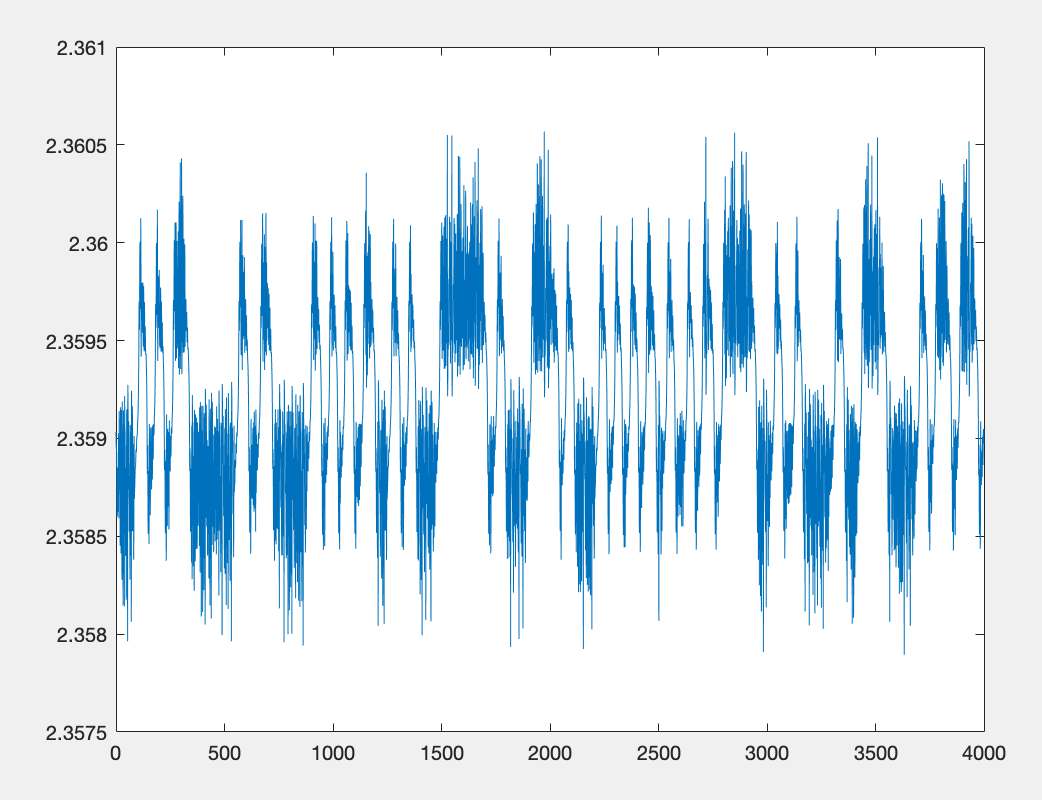
\includegraphics[width=0.9\linewidth]{senergy.png}
  \caption{Energy of the trajectory over time}
  \label{fig:sub1}
\end{subfigure}%
\begin{subfigure}{.5\textwidth}
  \centering
  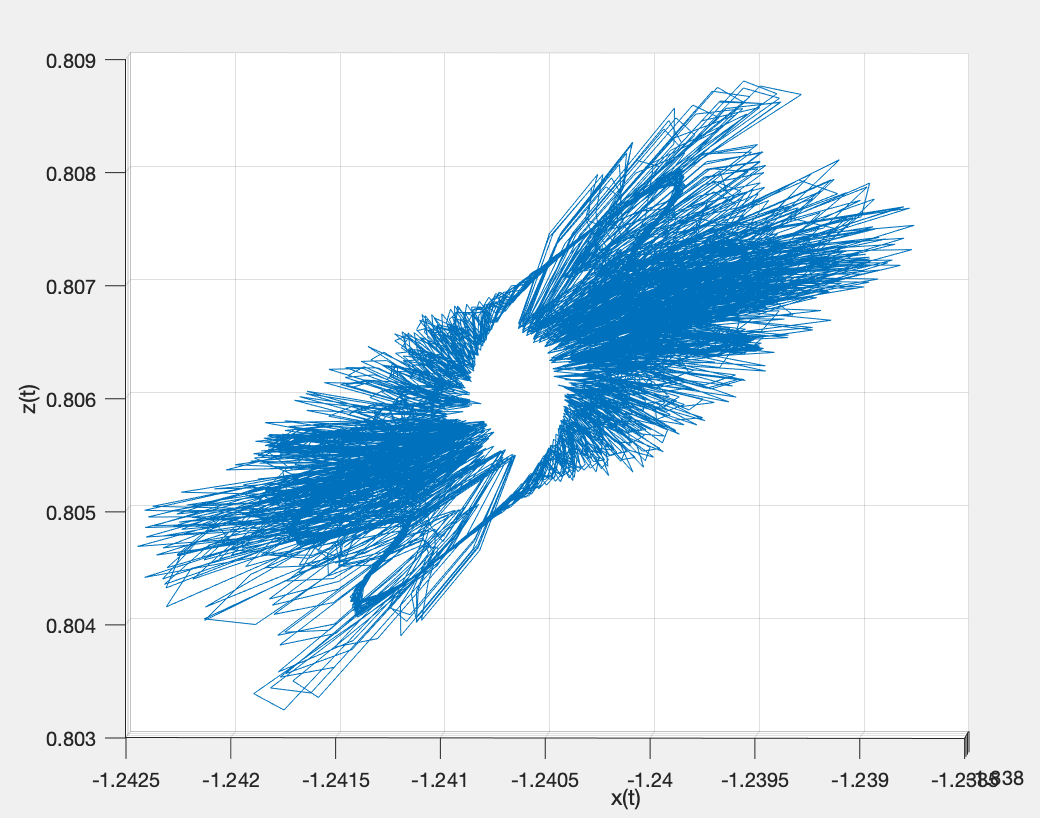
\includegraphics[width=0.92\linewidth]{splot.png}
  \caption{Plot of trajectory}
  \label{fig:sub2}
\end{subfigure}
\caption{}
\label{fig:une}
\end{figure}

The numerics in this case were not expected. In previous plots of both the elliptic and hyperbolic systems if a solution remained bounded it entered a fixed point and reached a steady state fixed point. The behavior in this case appears bounded and non periodic. It is possible that this result is only due to an error of MATLAB for such precise numerical values on a small scale. Either way, in the future I would like to continue studying this specific case and find if analysis agrees with the plots. 

With the presence of fixed points near the origin, one may assume that initial conditions far from the fixed point will always diverge. This is not the case as the forcing in the positive $y$-direction is what drives the divergence, and if we begin at a high energy with a $y_0 < 0$, in order to diverge the solution must travel to the other side of the $y$-axis, thus passing the fixed point and falling into a bounded steady state. We numerically show this with the same parameters as before, but now with $(x_0, y_0, z_0) = (-10, -100, 12)$. The numerics support boundedness in figure \ref{fig:new2}

\begin{figure}[h!]
\centering
\begin{subfigure}{.5\textwidth}
  \centering
  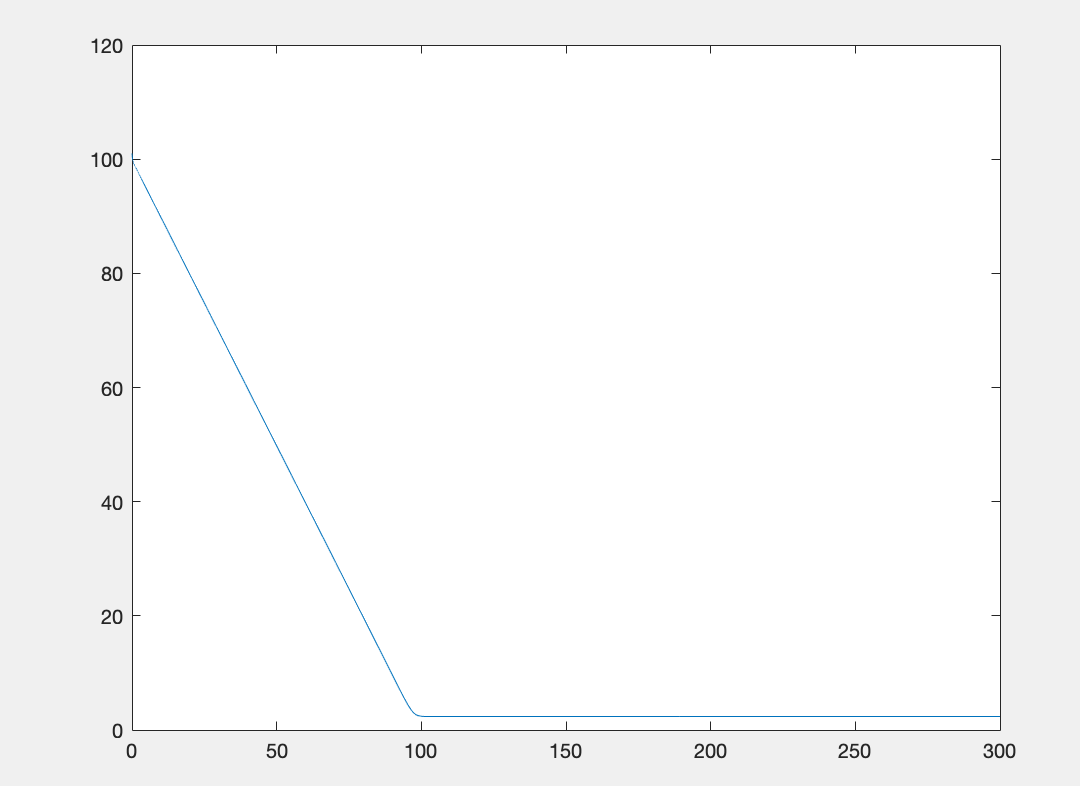
\includegraphics[width=0.9\linewidth]{new2e.png}
  \caption{Energy of the trajectory over time}
  \label{}
\end{subfigure}%
\begin{subfigure}{.5\textwidth}
  \centering
  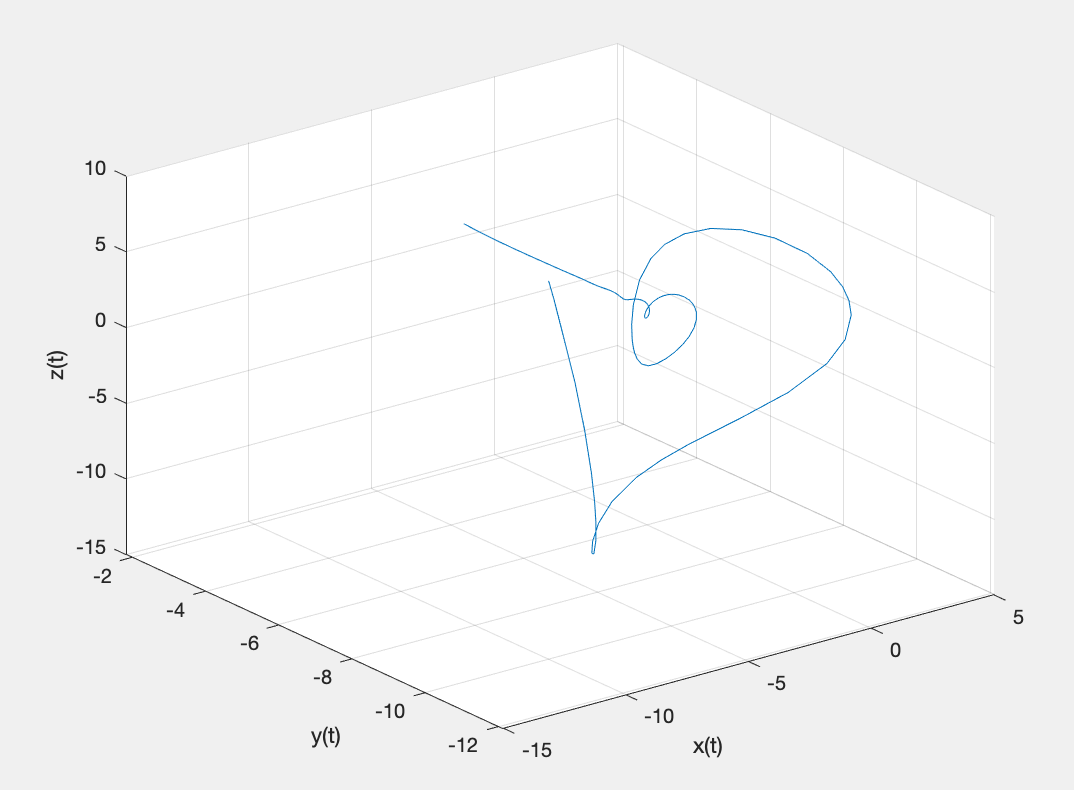
\includegraphics[width=0.9\linewidth]{new2p.png}
  \caption{Plot of trajectory}
  \label{}
\end{subfigure}
\caption{}
\label{fig:new2}
\end{figure}
Similar to the hyperbolic case, the trajectory for $y_0 > 0$ seemingly finds the stable fixed point near the origin. Now to show that it is the negative initial $y$ condition that led to convergence to a fixed point in the previous example, we can run the same simulation with a flipped $y_0$ in the initial conditions. Defining the initial conditions $(x_0, y_0, z_0) = (-10, 100, 12)$, the numerics for a short time show that the solution finds an invariant set in the $y$-axis and diverges towards $\underset{t \rightarrow \infty}{\lim}y(t) = +\infty$. Supporting plots are in figure \ref{fig:new3} below.


\begin{figure}[h!]
\centering
\begin{subfigure}{0.5\textwidth}
  \centering
  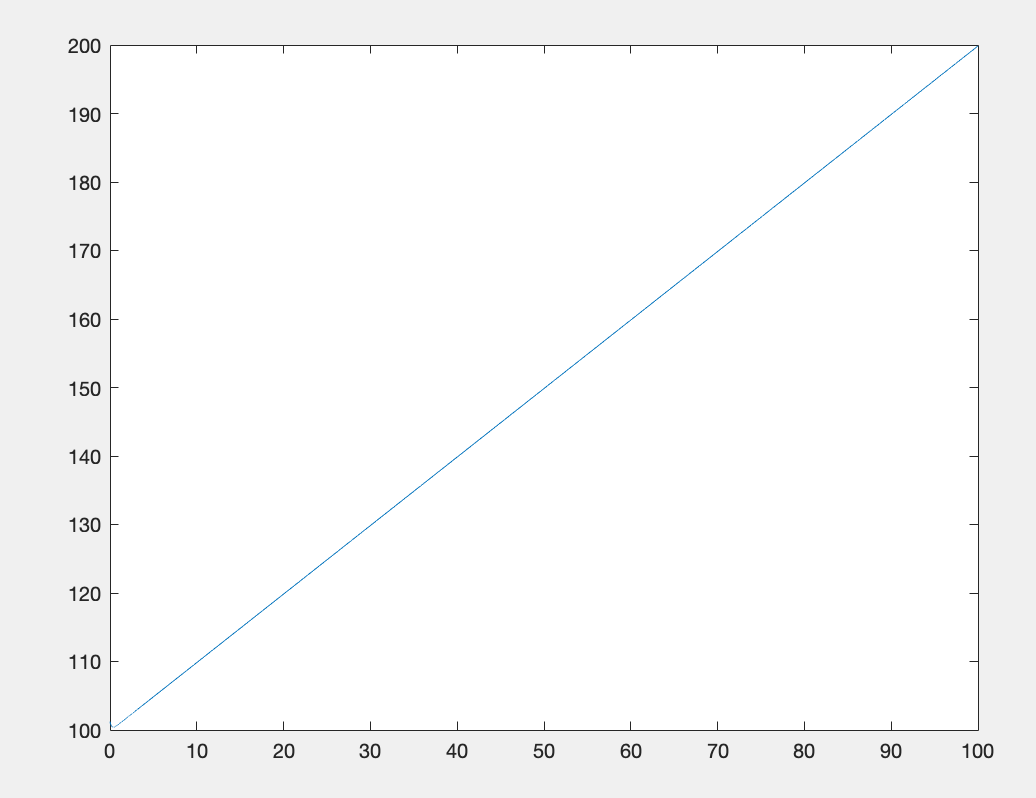
\includegraphics[width=0.93\linewidth]{new3e.png}
  \caption{Energy of the trajectory over time}
  \label{}
\end{subfigure}%
\begin{subfigure}{0.5\textwidth}
  \centering
  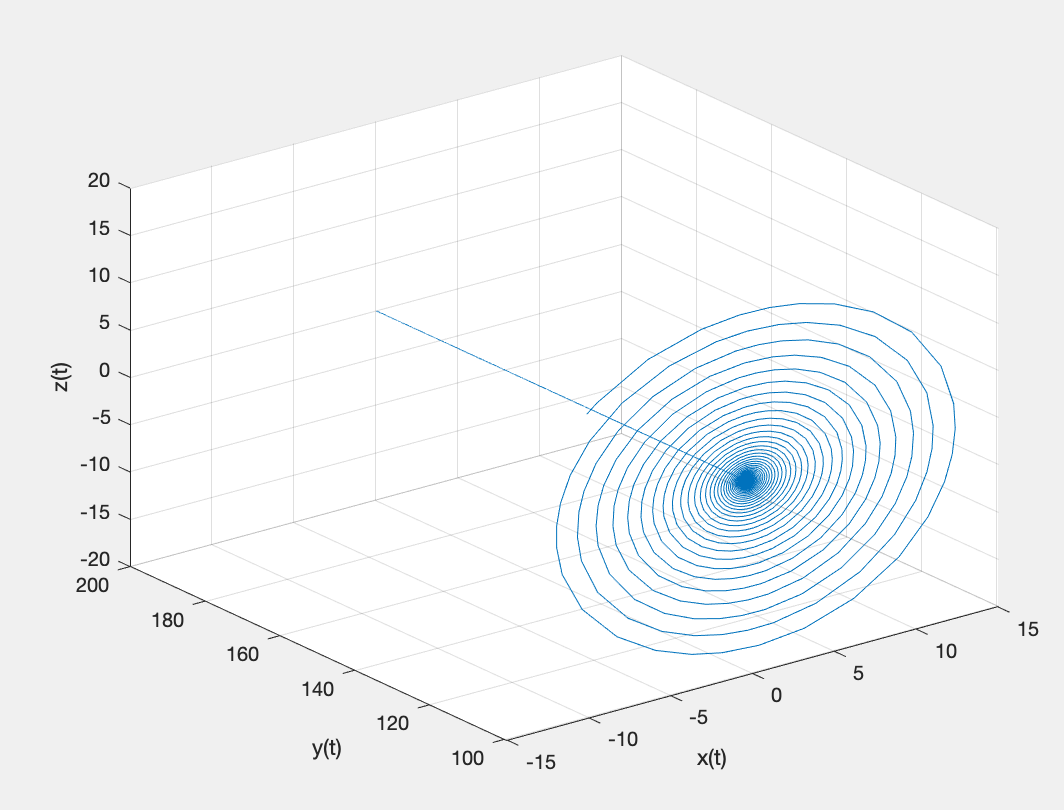
\includegraphics[width=0.93\linewidth]{new3p.png}
  \caption{Plot of trajectory}
  \label{}
\end{subfigure}
\caption{}
\label{fig:new3}
\end{figure}

However, letting our $y_0 < 0$ does not always necessitate boundedness. When we consider very negative initial $y$ conditions, we notice interesting behavior. An example, when we have the identical parameters as before, is for $(x_0, y_0, z_0) = (-1000, -1000, 1000)$. The behavior is shown below in figure \ref{fig:new1}

\begin{figure}[h!]
\centering
\begin{subfigure}{.462\textwidth}
  \centering
  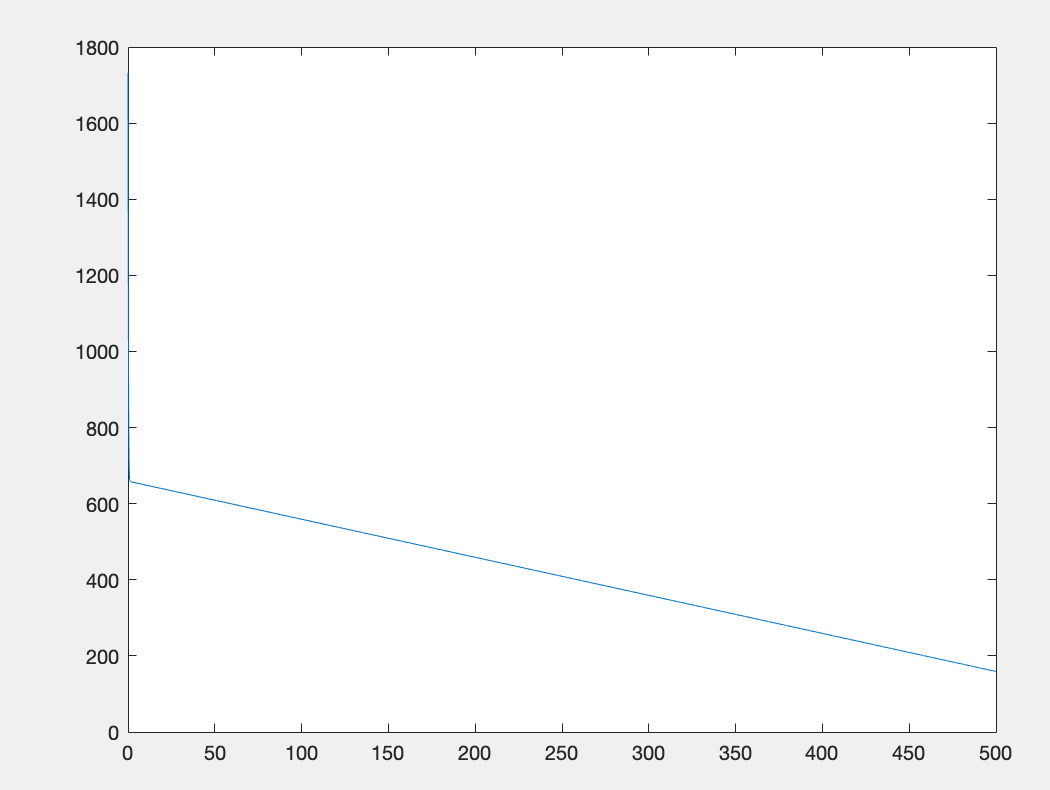
\includegraphics[width=1\linewidth]{new1e.png}
  \caption{Energy of the trajectory over time}
  \label{}
\end{subfigure}%
\begin{subfigure}{.5\textwidth}
  \centering
  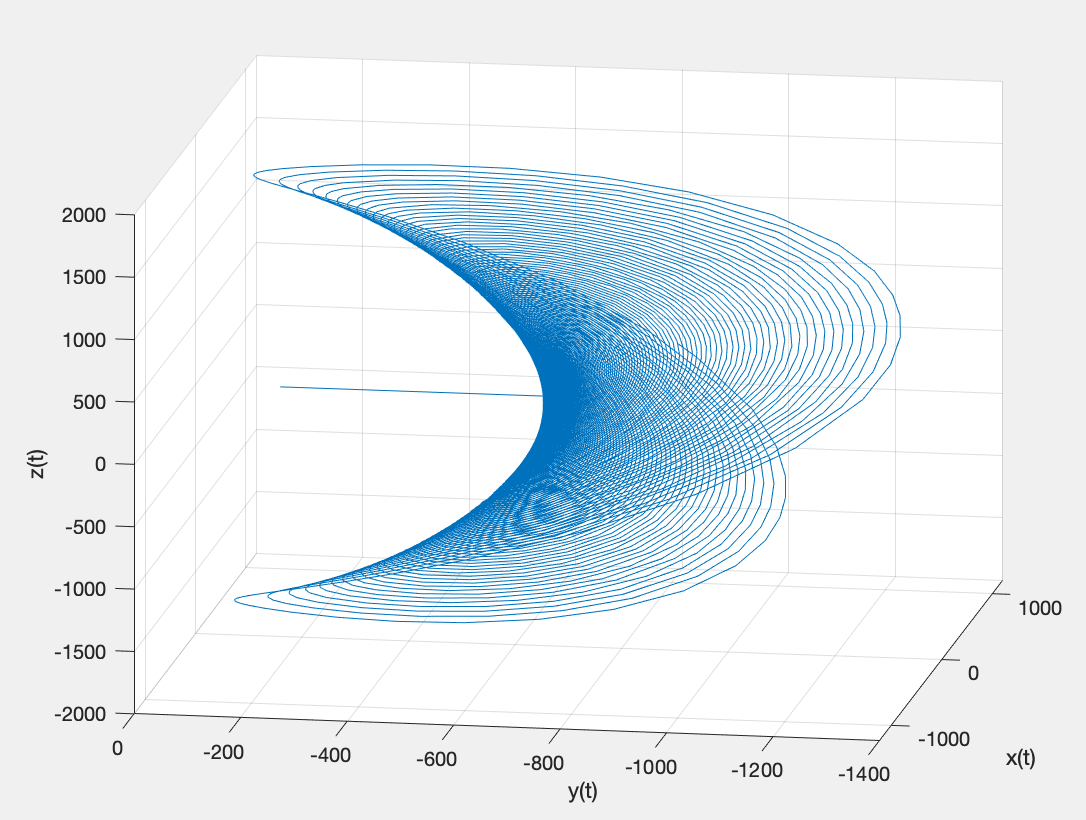
\includegraphics[width=0.92\linewidth]{new1p.png}
  \caption{Plot of trajectory}
  \label{}
\end{subfigure}
\caption{}
\label{fig:new1}
\end{figure}

The trajectory oscillates at very high energies and then seemingly approaches a stable fixed point, but when it reaches the $y$-axis, the elliptical conservative term keeps the trajectory in the kernel of $A$ and it diverges in the positive $y$ direction along the $y$-axis. After completing the approximation argument for the hyperbolic case, I would like to study the elliptic case in more detail. 


\end{document}
